% =============================================================================
% Introduction to Molecular Simulation --- Beamer deck (sbs_dark_beamer v10)
% 0 errors, 0 warnings target --- shell-escape for minted
% =============================================================================
\documentclass[aspectratio=169,10pt]{beamer}
% --- Font size increased per user request (8pt -> 10pt base) ---
\usepackage{sbs_dark_beamer}
\hfuzz=500pt\vfuzz=500pt\hbadness=10000\vbadness=10000
\usepackage{mwe} % for placeholder images if needed

% Additional TikZ libs for diagrams (already calc,shadows.blur etc loaded)
\usetikzlibrary{positioning,arrows.meta,shapes.geometric,fit,backgrounds,decorations.markings,patterns}

% Robust meme macro --- simple, no TikZ fallback to avoid extra }
\newcommand{\memeinclude}[2][width=0.85\linewidth]{%
  \IfFileExists{#2}{\includegraphics[#1]{#2}}{\fbox{\parbox{0.8\linewidth}{\centering\color{softgray}\tiny Meme: \texttt{#2} --- run \texttt{python scripts/generate\_meshy\_memes.py}}}}%
}

% Venn helper — dark text on light circles (FIXED white-on-white, removed blend group)
\newcommand{\venn}[3]{%
  \begin{tikzpicture}[scale=1.3]
      \fill[accentcyan!50,opacity=0.7] (0,0) circle (1.3cm);
      \fill[neonpink!50,opacity=0.7] (1.8,0) circle (1.3cm);
      \fill[neongreen!50,opacity=0.7] (0.9,1.5) circle (1.3cm);
    \node[color=bgblack] at (0,0) {\normalsize\bfseries #1};
    \node[color=bgblack] at (1.8,0) {\normalsize\bfseries #2};
    \node[color=bgblack] at (0.9,1.5) {\normalsize\bfseries #3};
  \end{tikzpicture}%
}

% Keyword interpretation box
\newcommand{\interpret}[1]{%
  \begin{successbox}[Interpretation --- keywords]
    \small #1
  \end{successbox}%
}

\graphicspath{{assets/}{assets/memes/}{./}}

\title{Introduction to Molecular Simulation}
\subtitle{From Bits to Bonds --- Computing Matter, One Atom at a Time}
\date{2026}
% Authors via sbs_dark_beamer mechanism
\clearauthors
\addauthor{Shuvam Banerji Seal}{IISER Kolkata}{shuvam@iiserkol.ac.in}

\begin{document}
% Disable auto section/subsection pages (they cause extra } with 16 sections)
\AtBeginSection[]{}
\AtBeginSubsection[]{}

% Title
\begin{frame}[plain]
	\titlepage
	\begin{center}
		
\includegraphics[height=1.2cm]{assets/figures/slashdot_logo.png}
	\end{center}
\end{frame}

% --- Video opener: YouTube-style thumbnail with play button (click opens new tab) ---
\begin{frame}{What is Simulation? --- 60s Primer}
	\begin{center}
		{\color{accentcyan}\normalsize\bfseries Click to watch: What is Simulation?}\par
		\vspace{0.3cm}
		\href{https://www.youtube.com/watch?v=XPE7eaR_XxM}{%
			\resizebox{0.88\linewidth}{!}{%
				\begin{tikzpicture}
					% 16:9 dark video player rectangle
					\fill[bgdark,rounded corners=4mm] (0,0) rectangle (11,6.19);
					\draw[accentcyan,rounded corners=4mm,line width=1.5pt] (0,0) rectangle (11,6.19);
					% Top red banner
					\fill[neonpink,rounded corners=4mm] (0,5.05) rectangle (11,6.19);
					\node[color=bgblack] at (5.5,5.62) {\large\bfseries What is Simulation?};
					% Center play button: red rounded rectangle + white triangle
					\fill[neonpink,rounded corners=3mm] (4.1,2.0) rectangle (6.9,3.6);
					\fill[white] (5.15,2.35) -- (5.15,3.25) -- (6.0,2.8) -- cycle;
					% Bottom URL bar
					\node[color=fgwhite] at (5.5,1.0) {\footnotesize\ttfamily youtube.com/watch?v=XPE7eaR\_XxM};
					\node[color=softgray] at (5.5,0.35) {\footnotesize click anywhere on this card to open in a new tab};
				\end{tikzpicture}%
			}%
		}\par
		\vspace{0.3cm}
		{\color{neonyellow}\normalsize\bfseries\href{https://www.youtube.com/watch?v=XPE7eaR_XxM}{[\,\,PLAY VIDEO\,\,\ensuremath{\rightarrow}\,]}}\par
	\end{center}
\end{frame}

% TOC --- two columns to hold all 16 sections
\begin{frame}{Outline --- Roadmap}
	\begin{multicols}{2}
		\footnotesize
		\tableofcontents[hideallsubsections]
	\end{multicols}
\end{frame}

% 16 Sections --- each input is a file in sections/
% 01 --- Introduction: Simulation / Modeling / Computational Experiments / Representation / Objectives / Applications
\section{Introduction to Molecular Simulation}

\subsection{What is Simulation?}
\begin{frame}{What is Simulation? --- Control Over Numbers on a Chip}
	\hfuzz=15pt
	\begin{columns}[T,onlytextwidth]
		\column{0.58\textwidth}
		\begin{pitemize}
			\item \neoncyan{Simulation} = computable mirror of reality
			\item \textbf{Control} \ensuremath{\rightarrow} numbers you \glow{ingrain} in silicon
			\item Chip = deterministic universe you design
			\item Input: \inlinecode{numbers} \ensuremath{\rightarrow} Output: \inlinecode{properties}
			\item \textbf{Why?} --- experiment impossible / dangerous / expensive
		\end{pitemize}
		\vspace{2mm}
		\begin{infobox}[Chip = Lab]
			\footnotesize Transistors \ensuremath{\rightarrow} arithmetic \ensuremath{\rightarrow} models \ensuremath{\rightarrow} atoms \ensuremath{\rightarrow} materials \ensuremath{\rightarrow} life
		\end{infobox}
		\column{0.45\textwidth}
		\begin{center}
			\begin{tikzpicture}[scale=0.92, every node/.style={font=\small}]
				% Chip with pins
				\node[draw=accentcyan,rounded corners=2mm,fill=darkgray,minimum width=3.2cm,minimum height=1.4cm,align=center,drop shadow={shadow xshift=0.5mm,shadow yshift=-0.5mm,opacity=0.5}] (chip) at (0,2.6) {\color{fgwhite}\bfseries\normalsize CPU/GPU\\\color{softgray}\footnotesize\ttfamily chip};
				% Chip pins — short stubs above and below the box only
				\foreach \x in {-1.0,-0.5,0,0.5,1.0} {\draw[accentcyan,thick] (\x,3.3) -- (\x,3.55); \draw[accentcyan,thick] (\x,1.9) -- (\x,1.65);}
				% Simulation
				\node[draw=neongreen,rounded corners=2mm,fill=bgdark,minimum width=3.5cm,minimum height=1.3cm,align=center,drop shadow] (sim) at (0,0.3) {\color{neongreen}\bfseries\normalsize Simulation\\\color{fgwhite}\footnotesize $F=ma$\,,\,$U(\mathbf{r})$};
				% Observables
				\node[draw=neonyellow,rounded corners=2mm,fill=bgdark,minimum width=3.5cm,minimum height=1.2cm,align=center,drop shadow] (obs) at (0,-2.0) {\color{neonyellow}\bfseries\normalsize Observables\\\color{fgwhite}\footnotesize $P,\ \rho,\ D,\ \Delta G$};
				% Arrows with labels
				\draw[-{Stealth[length=4mm,width=3mm]},thick,accentcyan] (chip.south) -- (sim.north) node[midway,right=8pt,font=\footnotesize,color=accentcyan]{model};
				\draw[-{Stealth[length=4mm,width=3mm]},thick,neongreen] (sim.south) -- (obs.north) node[midway,right=8pt,font=\footnotesize,color=neongreen]{measure};
				\only<2>{\node[draw=neonpink,fill=neonpink!12,rounded corners=2mm,inner sep=2.5mm,align=center] at (0,4.0) {\color{neonpink}\bfseries\small you control $\Delta t,\,T,\,P$!\\\color{bgblack}\footnotesize\ttfamily dt, thermostat, barostat};}
				\only<3>{\node[draw=accentcyan,fill=accentcyan!10,rounded corners=1mm,inner sep=2mm,align=center] at (3.2,0.3) {\color{accentcyan}\footnotesize\bfseries $10^9$ steps $\to$ $1\,\mu$s};}
			\end{tikzpicture}
		\end{center}
	\end{columns}
\end{frame}

\begin{frame}{Interpretation --- Simulation}
	\interpret{
		\textbf{Simulation} · mimic reality in code · \textbf{control} numbers \ensuremath{\rightarrow} control physics · \textbf{chip} = lab · \textbf{reproducible} · \textbf{cheap} \textit{what-if} · \textbf{not} magic --- model quality = result quality
	}
\end{frame}

\subsection{Molecular Modeling \& Orbital Concepts}
\begin{frame}{Molecular Modeling --- From Orbitals to Atoms}
	\begin{columns}[T,onlytextwidth]
		\column{0.55\textwidth}
		\begin{pitemize}
			\item \neoncyan{Orbitals} $\psi_{n\ell m}$ \ensuremath{\rightarrow} electron density
			\item Hydrogenic: $ \hat H\psi = E\psi $, $\psi_{100}\propto e^{-r/a_0}$
			\item Atoms \ensuremath{\rightarrow} \textbf{bonds}, \textbf{angles}, \textbf{dihedrals}
			\item Models: \textbf{Quantum} (DFT) vs \textbf{Classical} (balls+springs)
			\item Precision ladder: \glowstrong{hydrogenic} \ensuremath{\rightarrow} DFT \ensuremath{\rightarrow} force field
		\end{pitemize}
		\column{0.45\textwidth}
		\begin{tikzpicture}[scale=1.0]
			\shade[ball color=neonblue!70] (0,0) circle (0.35cm); \node[color=white] at (0,0){H};
			\shade[ball color=neongreen!70] (1.2,0.6) circle (0.28cm); \node[color=white] at (1.2,0.6){H};
			\shade[ball color=neonpink!70] (1.2,-0.6) circle (0.32cm); \node[color=white] at (1.2,-0.6){O};
			\draw[thick,accentcyan] (0,0) -- (1.2,0.6); \draw[thick,accentcyan] (0,0) -- (1.2,-0.6);
			\draw[dashed,neonyellow] (1.2,0.6) arc (60:-60:0.7cm);
			\node[color=neonyellow] at (1.8,0) {$\theta$};
			\only<2>{\draw[accentcyan,thick,dashed] (0.4,0.9) -- (0.4,1.6) node[above,color=accentcyan]{orbital cloud};}
		\end{tikzpicture}
		\vspace{2mm}
		{\footnotesize\color{softgray} Wireframe $\leftrightarrow$ Ball-and-stick $\leftrightarrow$ Space-filling}
	\end{columns}
\end{frame}

\begin{frame}{Interpretation --- Modeling}
	\interpret{
		\textbf{Modeling} · choose resolution · \textbf{orbitals} = quantum truth · \textbf{atoms} = classical shortcut · \textbf{precision} costs · \textbf{ball-and-stick} = human eye model
	}
\end{frame}

\subsection{Computational Experiments}
\begin{frame}{Computational Experiments --- The Third Pillar}
	\begin{columns}[T,onlytextwidth]
		\column{0.5\textwidth}
		\venn{Theory}{Experiment}{Simulation}
		\column{0.5\textwidth}
		\begin{pitemize}
			\item \textbf{Theory} \ensuremath{\rightarrow} equations
			\item \textbf{Experiment} \ensuremath{\rightarrow} nature answers
			\item \textbf{Simulation} \ensuremath{\rightarrow} \glow{nature under your conditions}
			\item Controlled $T,P,N$, perfect observation
			\item Falsifiable, reproducible
		\end{pitemize}
	\end{columns}
	\vspace{3mm}
	\begin{alertbox}[Not a video game]
		\footnotesize You don't watch molecules --- you \textbf{measure} them: $g(r)$, MSD, $\Delta G$.
	\end{alertbox}
\end{frame}

\subsection{Molecular Representation}
\begin{frame}{Molecular Representation --- How Computers See Molecules}
	\begin{columns}[T,onlytextwidth]
		\column{0.5\textwidth}
		\begin{pitemize}
			\item \textbf{Ball-and-stick}: atoms=spheres, bonds=sticks
			\item \textbf{Wireframe}: bonds only --- topology
			\item \textbf{Space-filling}: vdW radii --- volume
			\item \textbf{Cartoon}: proteins \ensuremath{\rightarrow} helices/sheets
			\item All derived from \inlinecode{coordinates + bonds}
		\end{pitemize}
		\column{0.5\textwidth}
		\memeinclude[width=0.9\linewidth]{assets/memes/water_meme.png}
		{\footnotesize\color{softgray} Meshy \texttt{nano-banana} --- water waving}
	\end{columns}
\end{frame}

\begin{frame}{Representation Zoo}
	\begin{columns}[T,onlytextwidth]
		\column{0.24\textwidth}
		\begin{center}
			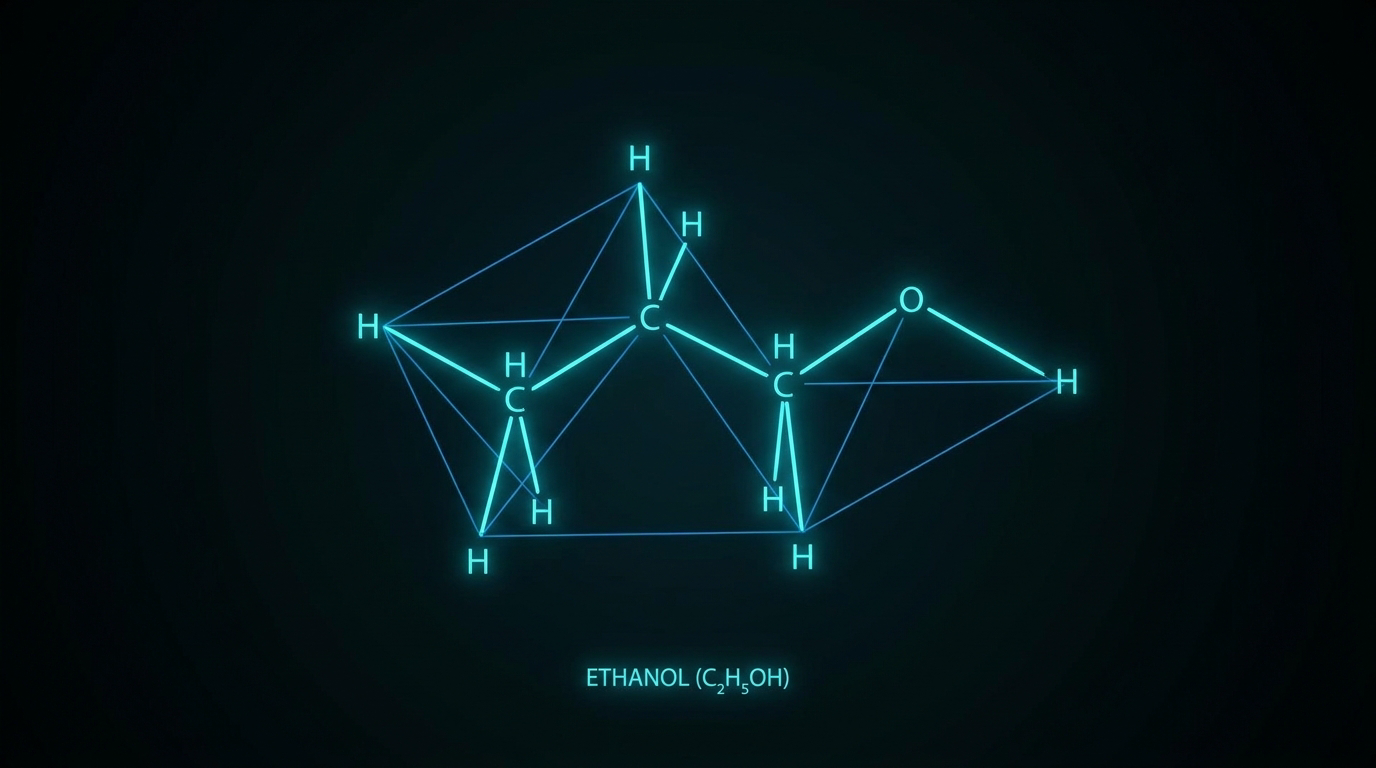
\includegraphics[width=\linewidth]{assets/figures/wireframe.png}
			{\footnotesize\color{softgray} Wireframe}
		\end{center}
		\column{0.24\textwidth}
		\begin{center}
			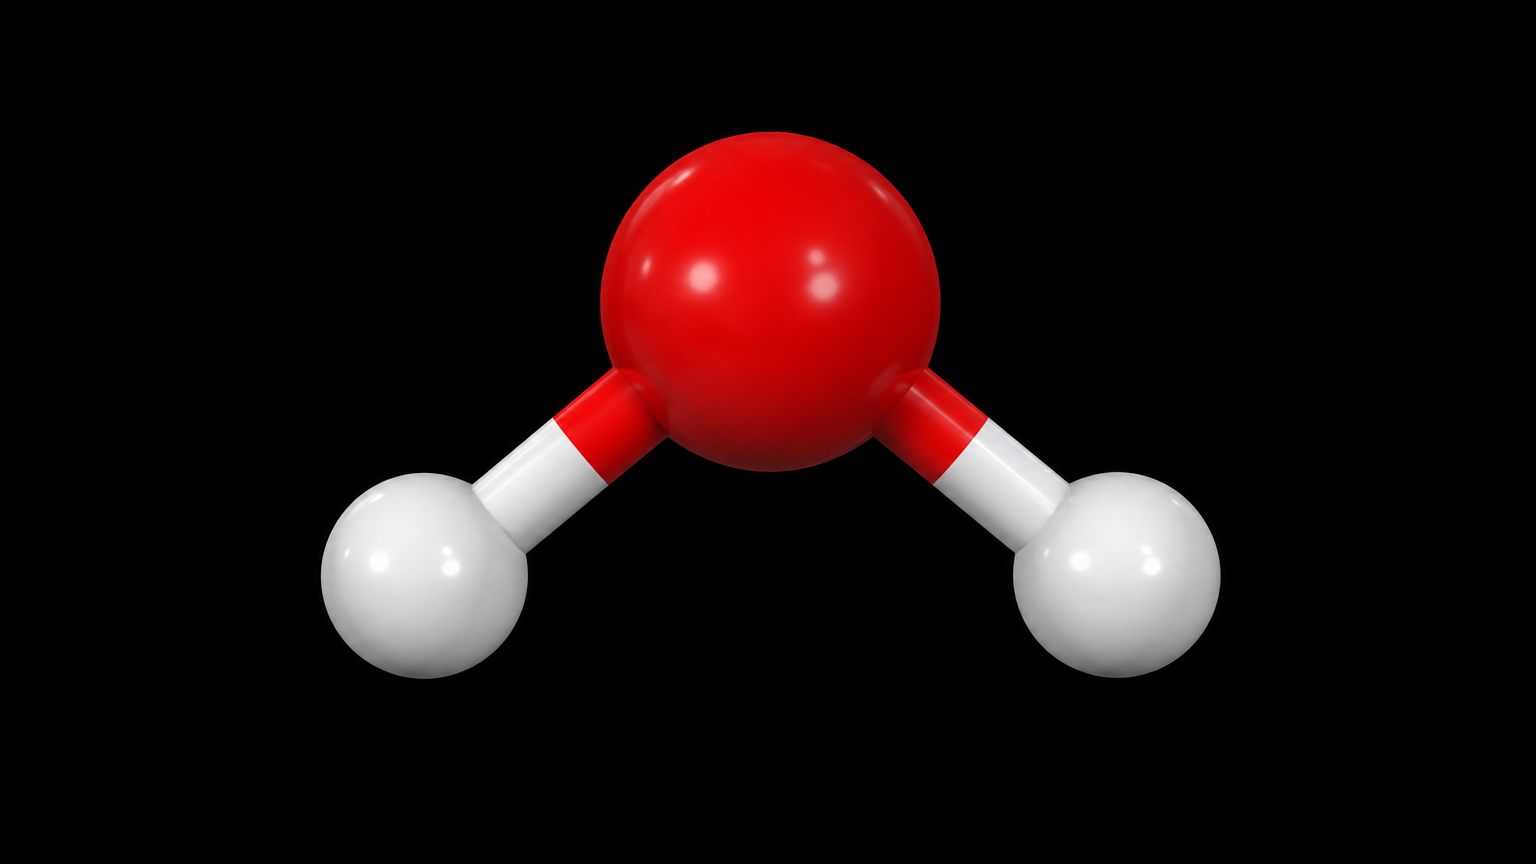
\includegraphics[width=\linewidth]{assets/figures/ball_stick_water.png}
			{\footnotesize\color{softgray} Ball-and-stick}
		\end{center}
		\column{0.24\textwidth}
		\begin{center}
			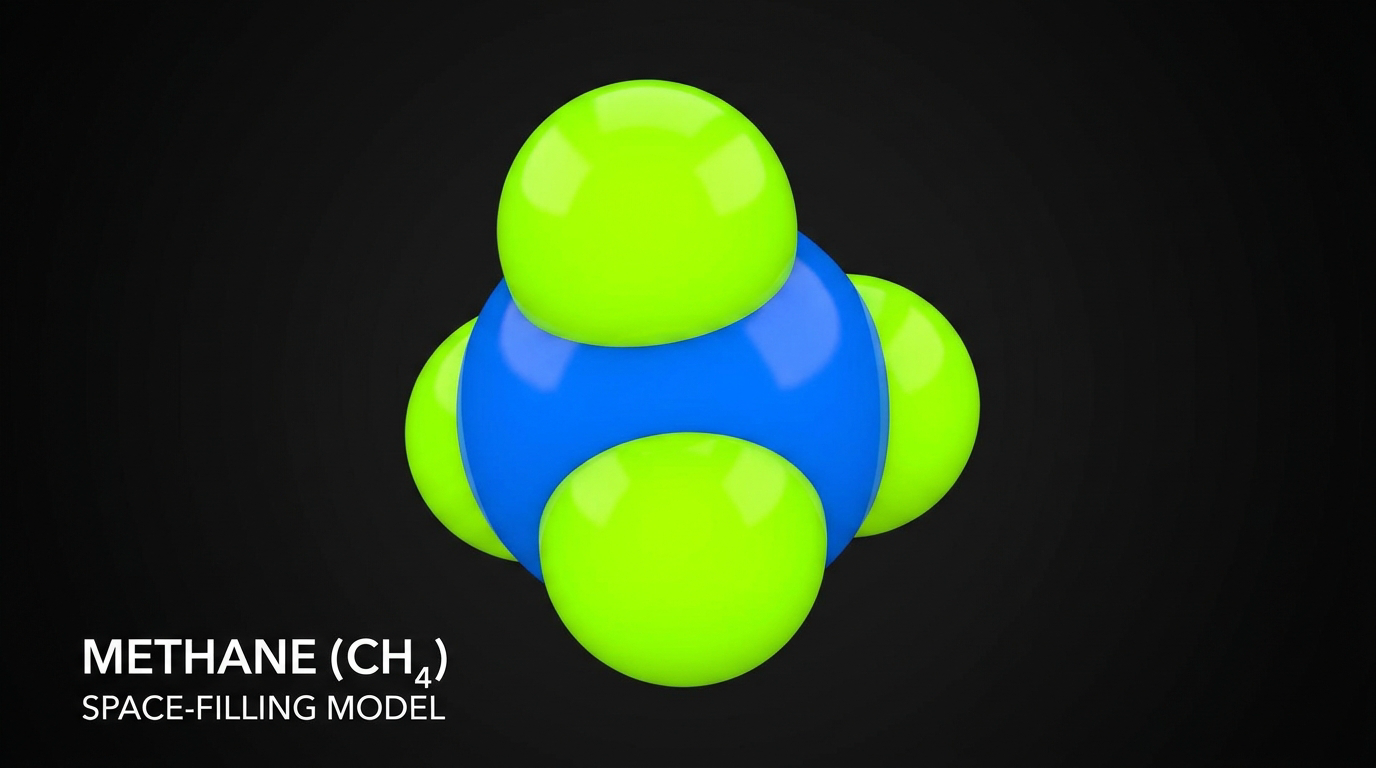
\includegraphics[width=\linewidth]{assets/figures/space_filling.png}
			{\footnotesize\color{softgray} Space-filling}
		\end{center}
		\column{0.24\textwidth}
		\begin{center}
			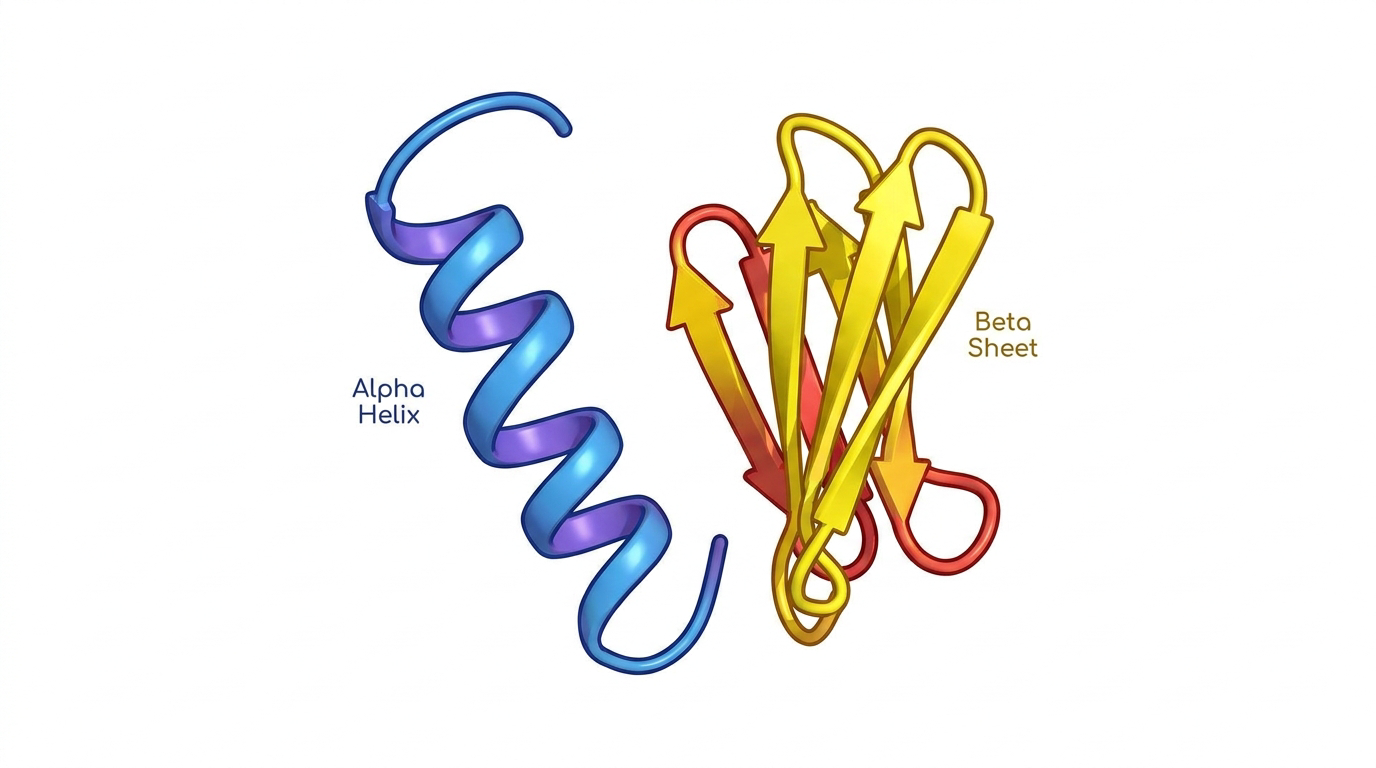
\includegraphics[width=\linewidth]{assets/figures/protein_cartoon.png}
			{\footnotesize\color{softgray} Cartoon}
		\end{center}
	\end{columns}
\end{frame}

\subsection{Objectives \& Applications}
\begin{frame}{Simulation Objectives --- What Are We After?}
	\begin{columns}[T,onlytextwidth]
		\column{0.5\textwidth}
		\begin{pitemize}
			\item \textbf{Structure}: $g(r)$, SASA, clustering
			\item \textbf{Dynamics}: $D$, $\tau$, rates
			\item \textbf{Thermodynamics}: $\Delta G$, $K_d$, phase
			\item \textbf{Mechanism}: pathway, $ PMF$
			\item \textbf{Design}: new molecule / material
		\end{pitemize}
		\column{0.5\textwidth}
		\begin{infobox}[Success = Question + Model + Sampling]
			\footnotesize Bad question + good model = noise\\\small Good question + bad model = \color{neonpink}lie
		\end{infobox}
		\vspace{2mm}
		\begin{tikzpicture}
			\node[draw=accentcyan,fill=accentcyan!15,rounded corners=1mm,inner sep=2mm,text=bgblack] {Drug binding \ensuremath{\rightarrow} Materials \ensuremath{\rightarrow} Energy \ensuremath{\rightarrow} Bio};
		\end{tikzpicture}
	\end{columns}
\end{frame}

\begin{frame}{Applications --- Where It Matters}
	\begin{columns}[T,onlytextwidth]
		\column{0.5\textwidth}
		\begin{pitemize}
			\item Pharma: binding $\Delta G$, \textbf{AlphaFold+MD}
			\item Materials: battery, polymer, catalyst
			\item Energy: CO2 capture, membranes
			\item Life: folding, crowding, rare events
		\end{pitemize}
		\column{0.5\textwidth}
		\memeinclude[width=0.95\linewidth]{assets/memes/intro_meme.png}
	\end{columns}
\end{frame}

\begin{frame}{Interpretation --- Objectives}
	\interpret{
		\textbf{Objectives} · \textbf{structure} / \textbf{dynamics} / \textbf{thermodynamics} · \textbf{mechanism} over movie · \textbf{design} is the test · \textbf{applications} drive approximations
	}
\end{frame}

% 02 --- Statistical Mechanics
\section{Statistical Mechanics}

\subsection{Microstates, Macrostates, Phase Space}
\begin{frame}{Microstate vs Macrostate}
	\begin{columns}[T,onlytextwidth]
		\column{0.5\textwidth}
		\begin{pitemize}
			\item \neoncyan{Microstate}: $\Gamma = \{ \mathbf{r}^N,\mathbf{p}^N\}$ --- everything
			\item \textcolor{neonpink}{Macrostate}: $(N,V,E)$ or $(N,P,T)$ --- few numbers
			\item One macro $\leftarrow$ many micro: $\Omega$ microstates
			\item Phase space: $6N$-dim, point = microstate
		\end{pitemize}
		\column{0.5\textwidth}
		\begin{center}
			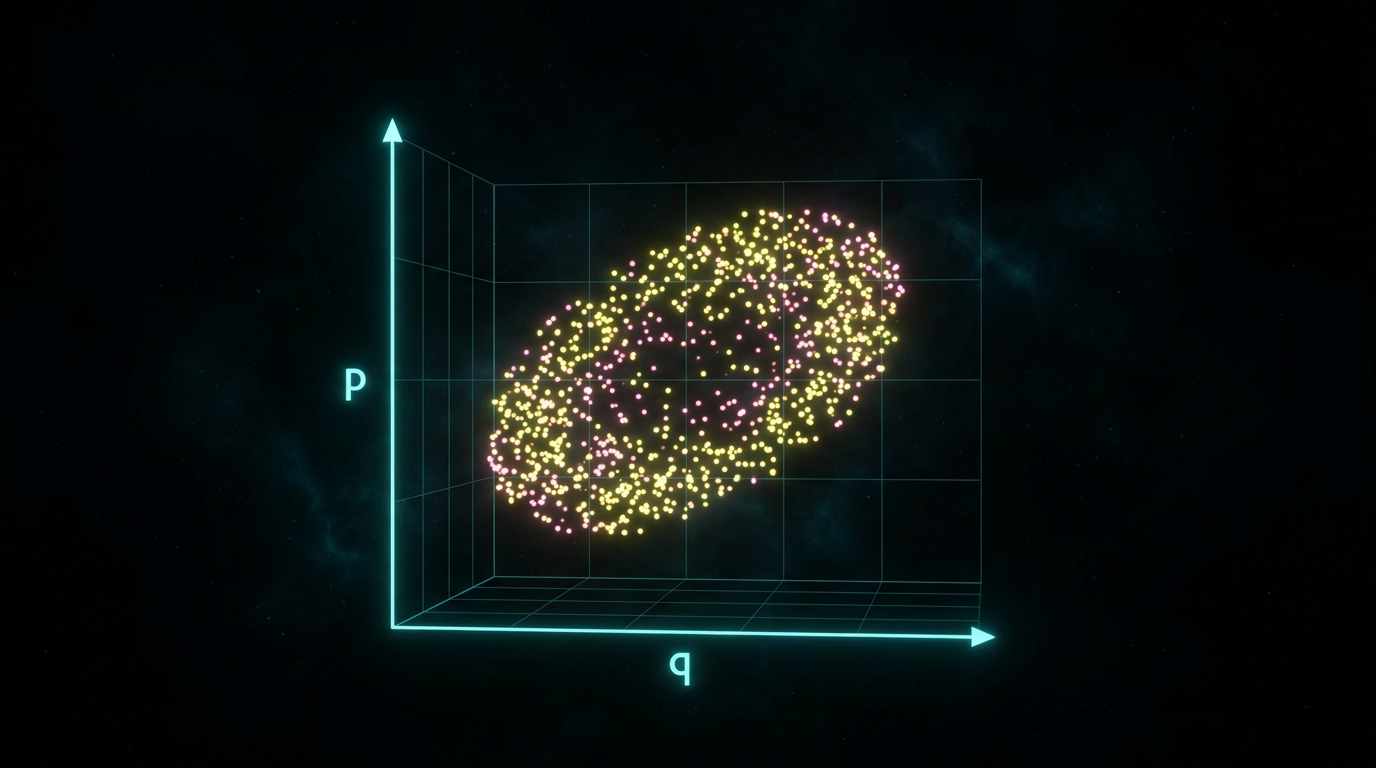
\includegraphics[width=0.9\linewidth]{assets/figures/phase_space.png}
			{\footnotesize\color{softgray} Phase space: each point = microstate}
		\end{center}
	\end{columns}
\end{frame}

\begin{frame}{Interpretation --- Micro/Macro}
	\interpret{
		\textbf{Micro} · exact positions·momenta · \textbf{macro} · thermometer numbers · \textbf{phase space} · map of all micros · \textbf{one macro} = \textbf{many micros}
	}
\end{frame}

\subsection{Energy, Entropy, Temperature}
\begin{frame}{Energy --- The Currency}
	\begin{equation*}
		E = K + U = \sum_i \frac{\mathbf{p}_i^2}{2m_i} + U(\mathbf{r}^N) \qquad \text{\color{softgray}\footnotesize micro definition}
	\end{equation*}
	\begin{columns}[T,onlytextwidth]
		\column{0.5\textwidth}
		\begin{pitemize}
			\item $U(\mathbf{r}^N)$ = PES --- see §3
			\item Conserved in NVE: $dE/dt=0$
			\item Fluctuates in NVT: $\langle (\Delta E)^2\rangle = k_BT^2 C_V$
		\end{pitemize}
		\column{0.5\textwidth}
		\begin{center}
			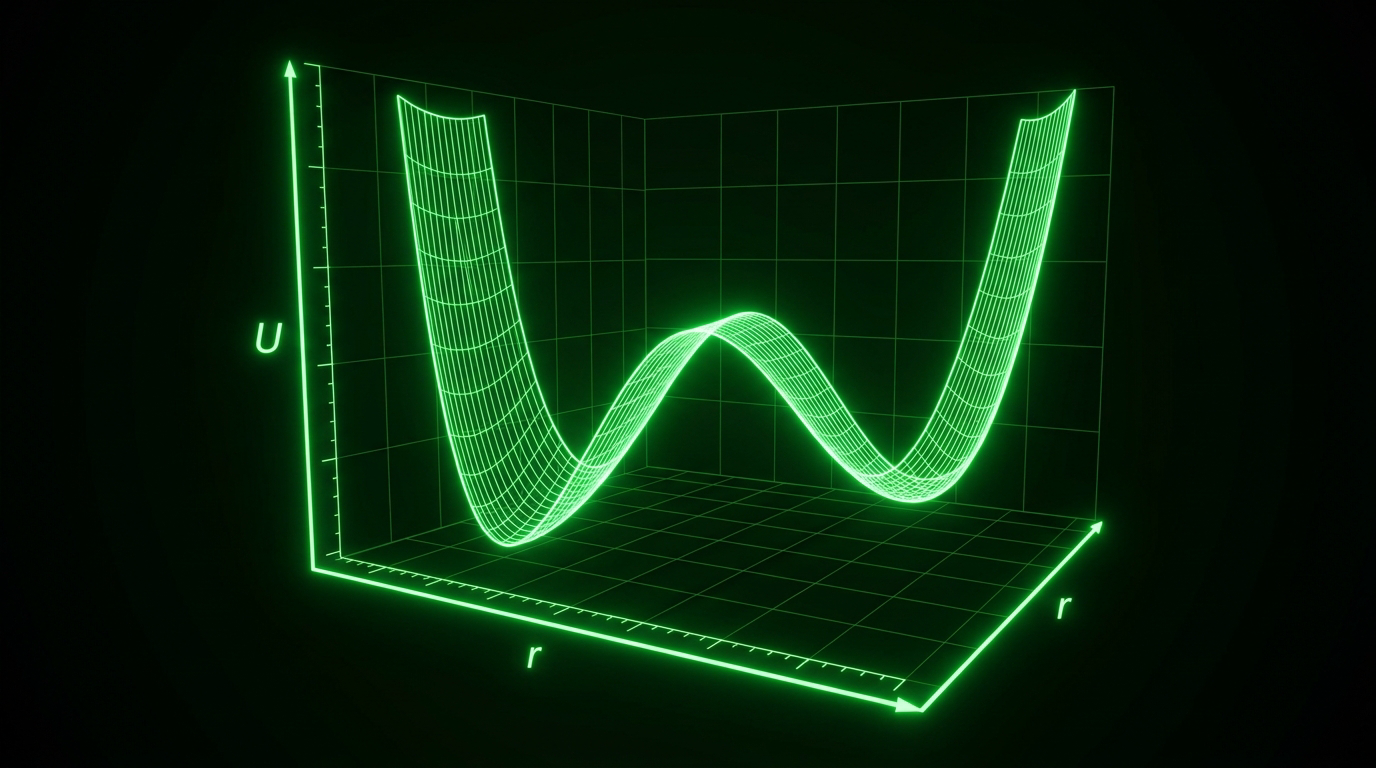
\includegraphics[width=0.9\linewidth]{assets/figures/energy_well.png}
			{\footnotesize\color{softgray} Potential energy $U(r)$: well + barrier}
		\end{center}
	\end{columns}
\end{frame}

\begin{frame}{Entropy --- Counting}
	\begin{equation*}
		S = k_B \ln \Omega \qquad\text{and}\qquad S = -k_B\sum_i p_i\ln p_i
	\end{equation*}
	\begin{columns}[T,onlytextwidth]
		\column{0.5\textwidth}
		\begin{pitemize}
			\item $\Omega$ = \# microstates for macro
			\item More ways \ensuremath{\rightarrow} more entropy \ensuremath{\rightarrow} more likely
			\item Disorder = \textbf{counting}, not mess
		\end{pitemize}
		\column{0.5\textwidth}
		\begin{center}
			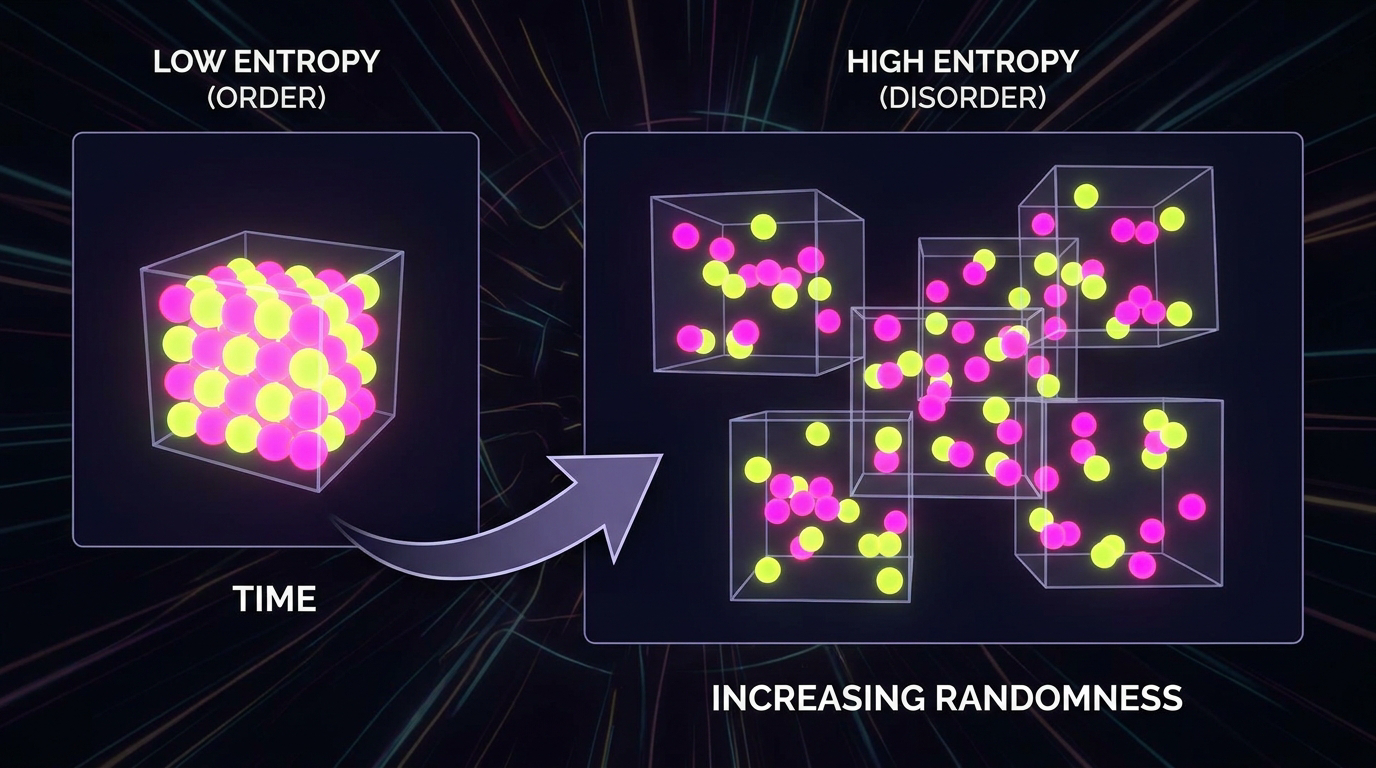
\includegraphics[width=0.9\linewidth]{assets/figures/entropy_counting.png}
			{\footnotesize\color{softgray} $\Omega=1$ (ordered) $\to$ $\Omega=10^{23}$ (disordered)}
		\end{center}
	\end{columns}
\end{frame}

\begin{frame}{Temperature --- Slope of Entropy}
	\begin{equation*}
		\frac{1}{T} = \left(\frac{\partial S}{\partial E}\right)_{N,V} \qquad
		\text{\color{softgray}hot = small slope}
	\end{equation*}
	\begin{columns}[T,onlytextwidth]
		\column{0.5\textwidth}
		\begin{pitemize}
			\item Cold: $S$ steep vs $E$
			\item Hot: $S$ flat vs $E$
			\item $T$ = \textbf{exchange rate} of $E \leftrightarrow S$
		\end{pitemize}
		\column{0.5\textwidth}
		\begin{tikzpicture}[scale=1.0]
			\draw[->,accentcyan] (0,0)--(2.8,0) node[right]{$E$};
			\draw[->,accentcyan] (0,0)--(0,2) node[above]{$S$};
			% Simple curve using coordinates instead of exp
			\draw[neongreen,thick] plot[smooth] coordinates {(0.2,0.2) (0.6,0.8) (1.0,1.2) (1.5,1.5) (2.0,1.7) (2.6,1.85)};
			\draw[dashed,neonyellow] (0.6,0) -- (0.6,0.8) -- (0,0.8);
			\node[color=neonyellow] at (0.6,-0.3) {cold $T$ low};
			\draw[dashed,neonpink] (2.0,0) -- (2.0,1.7) -- (0,1.7);
			\node[color=neonpink] at (2.0,-0.3) {hot $T$ high};
		\end{tikzpicture}
	\end{columns}
\end{frame}

\begin{frame}{Interpretation --- Energy/Entropy/Temperature}
	\interpret{
		\textbf{Energy} · conserved currency · \textbf{entropy} · count of ways · \textbf{temperature} · $dS/dE$ · \textbf{hot} = flat $S(E)$
	}
\end{frame}

\subsection{Free Energy \& Boltzmann}
\begin{frame}{Free Energy --- What Actually Matters}
	\begin{equation*}
		F = U - TS \qquad G = H - TS \qquad \min F,G \Leftrightarrow \text{stable}
	\end{equation*}
	\begin{columns}[T,onlytextwidth]
		\column{0.5\textwidth}
		\begin{pitemize}
			\item $U$ wants order, $S$ wants disorder
			\item $F$ = compromise at $T$
			\item Spontaneous $\Delta F<0$
		\end{pitemize}
		\column{0.5\textwidth}
		\memeinclude[width=0.95\linewidth]{assets/memes/boltzmann_meme.png}
	\end{columns}
\end{frame}

\begin{frame}{Boltzmann Distribution}
	\begin{equation*}
		p_i = \frac{e^{-\beta E_i}}{Z},\quad \beta=\frac1{k_BT},\quad Z=\sum_i e^{-\beta E_i}
	\end{equation*}
	\begin{columns}[T,onlytextwidth]
		\column{0.5\textwidth}
		\begin{pitemize}
			\item Low $E$ \ensuremath{\rightarrow} high $p$
			\item High $T$ \ensuremath{\rightarrow} flatter $p$
			\item $Z$ = partition function = normalization + \textbf{generator}
		\end{pitemize}
		\column{0.5\textwidth}
		\begin{center}
			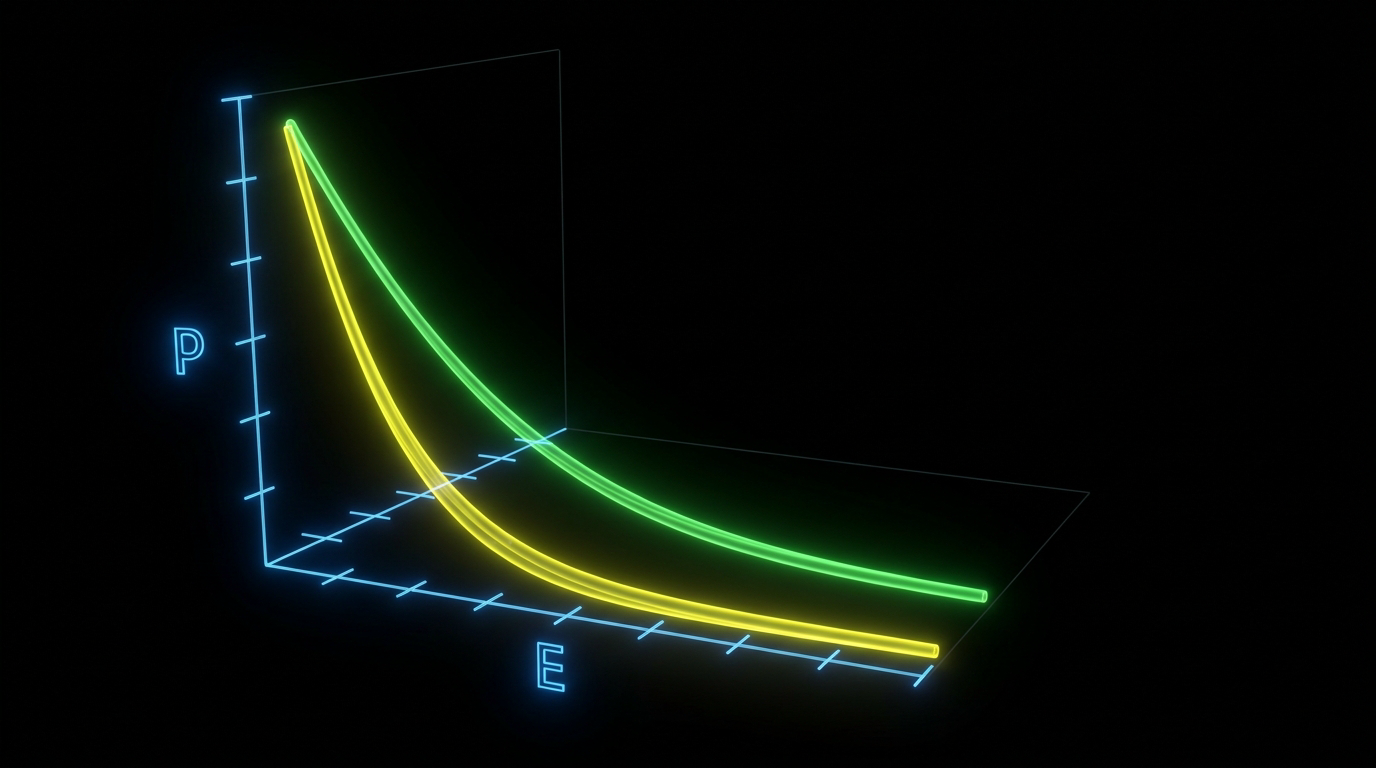
\includegraphics[width=0.9\linewidth]{assets/figures/boltzmann_dist.png}
			{\footnotesize\color{softgray} Boltzmann: cold (steep) vs hot (flat)}
		\end{center}
	\end{columns}
\end{frame}

\begin{frame}{Partition Function}
	\begin{equation*}
		Z = \sum e^{-\beta E} \;( \text{or } \int e^{-\beta H} d\Gamma ) \qquad
		F = -k_BT\ln Z
	\end{equation*}
	\begin{pitemize}
		\item $Z$ \ensuremath{\rightarrow} $F$ \ensuremath{\rightarrow} $P$, $S$, $C_V$ by derivatives
		\item Never need absolute $Z$, need \textbf{ratios} \ensuremath{\rightarrow} \textbf{sampling}
	\end{pitemize}
\end{frame}

\begin{frame}{Interpretation --- Free Energy/Boltzmann}
	\interpret{
		\textbf{free energy} · balance $U$ vs $TS$ · \textbf{Boltzmann} · low $E$ wins · \textbf{$Z$} · sum that rules them all · \textbf{cold} = picky, \textbf{hot} = tolerant
	}
\end{frame}

\subsection{Ensembles \& Ergodicity}
\begin{frame}{NVE, NVT, NPT --- Choose Your Lab}
	\begin{center}
		\begin{tikzpicture}[scale=1.0]
			\foreach \idx/\lab/\fix in {0/NVE/$E$,1/NVT/$T$,2/NPT/{$T,P$}} {
			\node[draw=accentcyan,rounded corners=2mm,fill=darkgray,minimum width=2.8cm,minimum height=1.4cm,align=center,font=\footnotesize] (b\idx) at (\idx*3.6,0) {\color{neonyellow}\bfseries \lab\\\color{fgwhite} fix \fix\\\color{softgray} micro/canonical/isobaric};
			}
			\draw[<->,thick,neongreen] (b0) -- (b1) node[midway,above,font=\footnotesize]{thermostat} ;
			\draw[<->,thick,neonpink] (b1) -- (b2) node[midway,above,font=\footnotesize]{barostat} ;
		\end{tikzpicture}
	\end{center}
	\begin{pitemize}
		\item \textbf{NVE}: isolated, $E$ conserved \ensuremath{\rightarrow} MD default
		\item \textbf{NVT}: heat bath, $T$ fixed \ensuremath{\rightarrow} biology lab
		\item \textbf{NPT}: $P$+ $T$ fixed \ensuremath{\rightarrow} real world
	\end{pitemize}
\end{frame}

\begin{frame}{Ergodicity \& Ensemble Average}
	\begin{equation*}
		\langle A\rangle = \sum_i A_i p_i \approx \frac1{T}\int_0^T A(t)\,dt \quad\text{if ergodic}
	\end{equation*}
	\begin{columns}[T,onlytextwidth]
		\column{0.5\textwidth}
		\begin{pitemize}
			\item \textbf{Ergodic}: trajectory visits all with correct weight
			\item Broken \ensuremath{\rightarrow} trapped, \textbf{rare events} matter
			\item Solution: \textbf{enhanced sampling} (§9)
		\end{pitemize}
		\column{0.5\textwidth}
		\begin{center}
			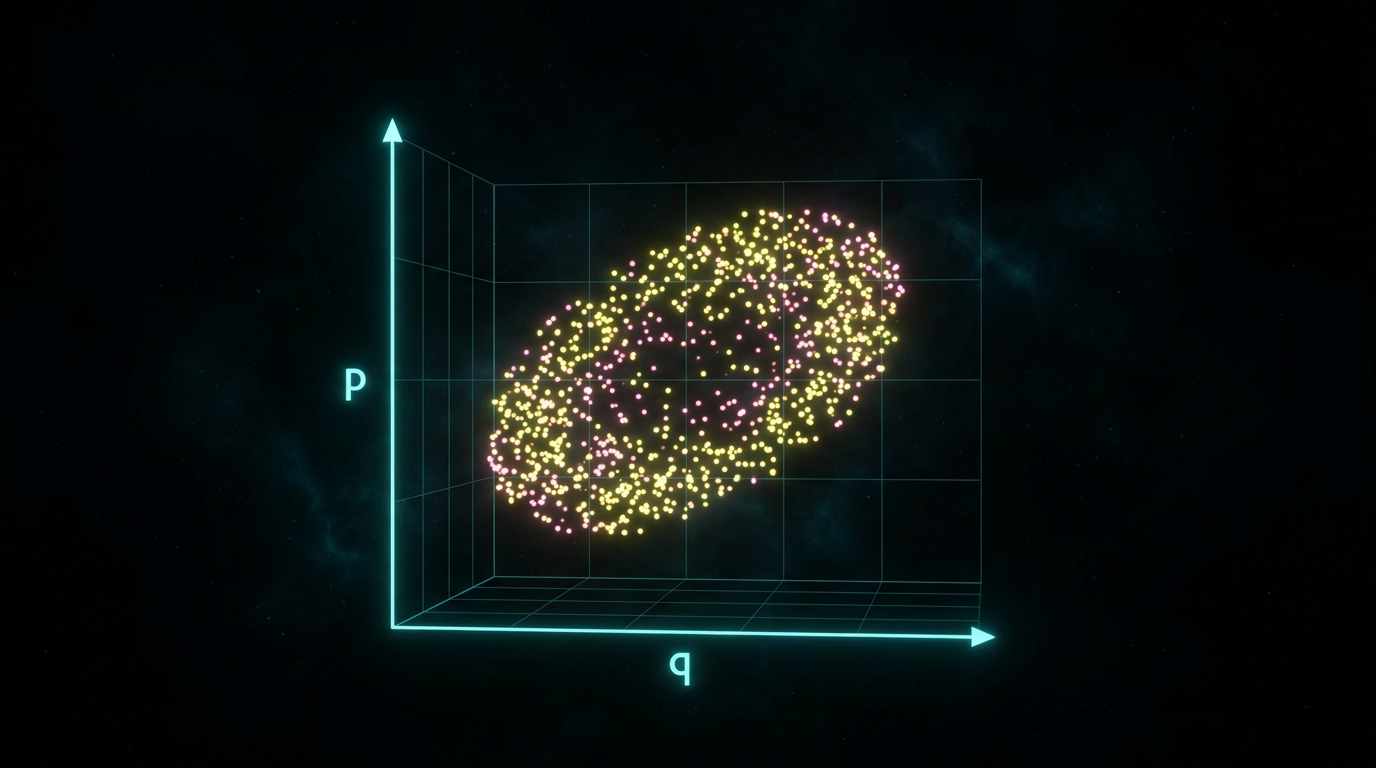
\includegraphics[width=0.9\linewidth]{assets/figures/phase_space.png}
			{\footnotesize\color{softgray} Trajectory (line) vs ensemble (shaded)}
		\end{center}
	\end{columns}
\end{frame}

\begin{frame}{Interpretation --- Ensembles}
	\interpret{
		\textbf{ensembles} · what you fix · \textbf{NVE/NVT/NPT} · lab choice · \textbf{ergodic} · time = ensemble · \textbf{broken} \ensuremath{\rightarrow} sample smarter
	}
\end{frame}

% 03 --- Molecular Representation on Computers (rigorous)
\section{Molecular Representation on Computers}

\subsection{Coordinates, Topology}
\begin{frame}{Atomic Coordinates --- The $3N$ Truth}
  \begin{equation*}
    \mathbf{R} = \{\mathbf{r}_1,\dots,\mathbf{r}_N\},\quad \mathbf{r}_i=(x_i,y_i,z_i)\in\mathbb{R}^3
  \end{equation*}
  \begin{columns}[T,onlytextwidth]
    \column{0.5\textwidth}
    \begin{pitemize}
      \item $3N$ numbers = \textbf{complete} classical description
      \item File: \inlinecode{XYZ / PDB / GRO} \ensuremath{\rightarrow} list
      \item Units: Å (most), nm (GROMACS)
      \item \textbf{Rigorous}: coordinates \textbf{are} the state
    \end{pitemize}
    \column{0.5\textwidth}
    \begin{center}
      \begin{tikzpicture}[scale=0.9]
        \node[draw=accentcyan,fill=darkgray,rounded corners=1mm,minimum width=2.6cm,minimum height=0.8cm] at (0,1) {\color{fgwhite}\tiny\ttfamily ATOM 1 C 0.0 0.0 0.0};
        \node[draw=accentcyan,fill=darkgray,rounded corners=1mm,minimum width=2.6cm,minimum height=0.8cm] at (0,0) {\color{fgwhite}\tiny\ttfamily ATOM 2 O 1.2 0.0 0.0};
        \node[draw=accentcyan,fill=darkgray,rounded corners=1mm,minimum width=2.6cm,minimum height=0.8cm] at (0,-1) {\color{fgwhite}\tiny\ttfamily ATOM 3 H -0.4 0.9 0.0};
        \draw[->,thick,neongreen] (1.4,1) -- (2.2,0.2) node[right,color=neongreen]{array};
      \end{tikzpicture}
    \end{center}
  \end{columns}
\end{frame}

\begin{frame}{Bonds, Angles, Dihedrals --- Topology}
  \begin{columns}[T,onlytextwidth]
    \column{0.5\textwidth}
    \begin{pitemize}
      \item \textbf{Bond}: $r_{ij}=|\mathbf{r}_j-\mathbf{r}_i|$ · 2 atoms
      \item \textbf{Angle}: $\theta_{ijk}$ · 3 atoms
      \item \textbf{Dihedral}: $\phi_{ijkl}$ · 4 atoms, \textbf{periodic}
      \item Topology = \textbf{graph} (bonds = edges)
    \end{pitemize}
    \column{0.5\textwidth}
    \begin{tikzpicture}[scale=0.9]
      \coordinate (A) at (0,0); \coordinate (B) at (1.2,0.6); \coordinate (C) at (2.4,0.2); \coordinate (D) at (3.2,1.1);
      \foreach \p in {A,B,C,D} {\shade[ball color=accentcyan] (\p) circle (0.22cm);}
      \draw[thick,white] (A)--(B)--(C)--(D);
      \draw[dashed,neonyellow] (A)--(C); \node[color=neonyellow] at (1.2,-0.4) {angle $\theta$};
      \draw[dashed,neonpink] (B)--(D); \node[color=neonpink] at (2.8,0.7) {dihedral $\phi$};
      \only<2>{\draw[->,thick,neongreen] (B) -- ++(0.4,0.8) node[above]{4-body!};}
    \end{tikzpicture}
  \end{columns}
\end{frame}

\begin{frame}{Interpretation --- Coordinates/Topology}
  \interpret{
    \textbf{coordinates} · $3N$ numbers = molecule · \textbf{bond} · distance · \textbf{angle} · 3 atoms · \textbf{dihedral} · 4 atoms = flexibility · \textbf{topology} · graph
  }
\end{frame}

\subsection{Masses, Charges, Box, PBC}
\begin{frame}{Masses \& Partial Charges}
  \begin{columns}[T,onlytextwidth]
    \column{0.5\textwidth}
    \begin{pitemize}
      \item $m_i$ \ensuremath{\rightarrow} dynamics: $\mathbf{F}=m\mathbf{a}$
      \item $q_i$ \ensuremath{\rightarrow} electrostatics: $U_{\text{Coul}}=\frac{q_iq_j}{4\pi\epsilon_0 r_{ij}}$
      \item \textbf{Partial} \ensuremath{\neq} formal: fitted to reproduce $ \Phi(\mathbf{r})$
      \item Rigorous: charges are \textbf{parameters}, not observables
    \end{pitemize}
    \column{0.5\textwidth}
    \begin{tikzpicture}[scale=0.9]
      \shade[ball color=neonblue] (0,0) circle (0.45cm) node[color=white]{O$^{-0.8}$};
      \shade[ball color=neonyellow] (-0.9,0.7) circle (0.32cm) node[color=bgblack]{H$^{+0.4}$};
      \shade[ball color=neonyellow] (0.9,0.7) circle (0.32cm) node[color=bgblack]{H$^{+0.4}$};
      \draw[->,thick,accentcyan] (0,-0.6) -- (0,-1.3) node[below,color=accentcyan]{$\mathbf{\mu}$};
    \end{tikzpicture}
  \end{columns}
\end{frame}

\begin{frame}{Simulation Box \& Periodic Boundary Conditions}
  \begin{columns}[T,onlytextwidth]
    \column{0.5\textwidth}
    \begin{pitemize}
      \item Box: $\mathbf{L}=(L_x,L_y,L_z)$, triclinic: $\mathbf{h}$
      \item \textbf{PBC}: infinite tiles, minimum image
      \item Rigorous: removes surface, \textbf{finite-size} remains
      \item Cutoff $r_c < L/2$ 
    \end{pitemize}
    \column{0.5\textwidth}
    \begin{center}
      \begin{tikzpicture}[scale=0.6]
        \draw[accentcyan,thick] (0,0) rectangle (1.8,1.4);
        % PBC images (simplified, no conditional)
        \foreach \dx in {-1.8,1.8} \foreach \dy in {-1.4,0,1.4} {
          \draw[softgray,thin] (\dx,\dy) rectangle ++(1.8,1.4); \fill[neonpink] (\dx+0.9,\dy+0.7) circle (1pt);
        }
        \foreach \dx in {0} \foreach \dy in {-1.4,1.4} {
          \draw[softgray,thin] (\dx,\dy) rectangle ++(1.8,1.4); \fill[neonpink] (\dx+0.9,\dy+0.7) circle (1pt);
        }
        \fill[accentcyan] (0.9,0.7) circle (2pt);
        \node[color=accentcyan] at (0.9,1.7) {central box};
        \draw[dashed,neonyellow] (0.9,0.7) -- (2.7,0.7) node[midway,above]{image};
      \end{tikzpicture}
    \end{center}
  \end{columns}
\end{frame}

\subsection{PES \& Force Fields}
\begin{frame}{Potential Energy Surface --- The Mountain Range}
  \begin{equation*}
    U(\mathbf{R}) : \mathbb{R}^{3N}\to\mathbb{R} \qquad \mathbf{F}_i = -\nabla_{\mathbf{r}_i}U
  \end{equation*}
  \begin{columns}[T,onlytextwidth]
    \column{0.5\textwidth}
    \begin{pitemize}
      \item $3N$-dim surface \ensuremath{\rightarrow} $2$D cartoon is \textbf{projection}
      \item Minima = stable structures
      \item Saddle = transition state
      \item Rigorous: \textbf{all} physics in $U$
    \end{pitemize}
    \column{0.5\textwidth}
    \begin{tikzpicture}[scale=0.6]
      \draw[accentcyan!50,fill=accentcyan!10] plot[smooth] coordinates {(0,0) (0.6,0.8) (1.2,0.3) (1.8,1.1) (2.4,0.6) (3,1.3)} -- (3,0) -- cycle;
      \fill[neongreen] (0.6,0.8) circle (2pt) node[above,color=neongreen]{min};
      \fill[neonpink] (1.8,1.1) circle (2pt) node[above,color=neonpink]{min};
      \fill[neonyellow] (1.2,0.3) circle (2pt) node[below,color=neonyellow]{saddle};
      \draw[->,thick,accentcyan] (1.2,0.3) -- (1.8,1.1) node[midway,sloped,above]{barrier};
    \end{tikzpicture}
  \end{columns}
\end{frame}

\begin{frame}{Force Fields --- $U$ Made Computable}
  \begin{equation*}
    U = \underbrace{U_{\text{bond}}+U_{\text{angle}}+U_{\text{dihed}}}_{\text{bonded}} + \underbrace{U_{\text{LJ}}+U_{\text{Coul}}}_{\text{nonbonded}}
  \end{equation*}
  \begin{columns}[T,onlytextwidth]
    \column{0.5\textwidth}
    \begin{pitemize}
      \item Bond: $k_b(r-r_0)^2$ · spring
      \item LJ: $4\epsilon[(\sigma/r)^{12}-(\sigma/r)^6]$
      \item Many: AMBER, CHARMM, OPLS, ReaxFF, \textbf{ML potentials}
    \end{pitemize}
    \column{0.5\textwidth}
    \begin{infobox}[FF = Expensive Physics Compressed]
      \scriptsize $10^5$ DFT points \ensuremath{\rightarrow} $U_{\text{FF}}$ \ensuremath{\rightarrow} $10^9$ steps
    \end{infobox}
  \end{columns}
\end{frame}

\begin{frame}{Interpretation --- PES/FF}
  \interpret{
    \textbf{PES} · energy landscape · \textbf{force} = slope · \textbf{force field} · cheap $U$ · \textbf{bonded + nonbonded} · \textbf{parameterized} \ensuremath{\rightarrow} not universal
  }
\end{frame}

% 04 --- Accuracy and Approximation (incl. IEEE 754)
\section{Accuracy and Approximation in Simulation}

\begin{frame}{Accuracy --- What Does \textit{Correct} Mean?}
	\begin{columns}[T,onlytextwidth]
		\column{0.5\textwidth}
		\begin{pitemize}
			\item \textbf{Accuracy} = closeness to \textbf{reality}
			\item Not vs. code, vs. \textbf{nature}
			\item Validate: $g(r)$, $D$, $\Delta G$ vs. experiment
			\item \textbf{Errors} stack: model + numerics + sampling
		\end{pitemize}
		\column{0.5\textwidth}
		\venn{Accuracy}{Precision}{Cost}
		\vspace{2mm}
		{\footnotesize\color{softgray} You can be precise and still wrong.}
	\end{columns}
\end{frame}

\subsection{Force-Field Approximations}
\begin{frame}{Force-Field Approximations}
	\begin{columns}[T,onlytextwidth]
		\column{0.55\textwidth}
		\begin{pitemize}
			\item Fixed topology \ensuremath{\rightarrow} no bond breaking (except ReaxFF)
			\item Pairwise $U_{\text{LJ}}$ \ensuremath{\rightarrow} no many-body
			\item Point charges \ensuremath{\rightarrow} no polarization (unless Amoeba/Drude)
			\item Harmonic bonds \ensuremath{\rightarrow} no anharmonicity at large $r$
		\end{pitemize}
		\column{0.45\textwidth}
		\begin{center}
			\begin{tikzpicture}[scale=1.0]
				% QM reality: bumpy curve
				\draw[->,accentcyan,thick] (0,0) -- (3.2,0) node[right]{$r$};
				\draw[->,accentcyan,thick] (0,0) -- (0,2.4) node[above]{$U$};
				% QM curve (bumpy, true)
				\draw[neonyellow,thick] plot[smooth] coordinates {(0.2,2.2) (0.5,1.8) (0.8,0.9) (1.1,0.5) (1.4,0.6) (1.7,0.9) (2.0,1.2) (2.4,1.5) (2.8,1.7) (3.0,1.8)};
				\node[color=neonyellow,font=\footnotesize] at (2.6,2.0) {QM (truth)};
				% FF curve (smooth, approximate)
				\draw[neonpink,thick,dashed] plot[smooth] coordinates {(0.2,2.1) (0.5,1.5) (0.8,0.7) (1.1,0.4) (1.4,0.45) (1.7,0.6) (2.0,0.8) (2.4,1.1) (2.8,1.4) (3.0,1.6)};
				\node[color=neonpink,font=\footnotesize] at (0.6,2.1) {FF (approx)};
				% Error arrows
				\draw[<->,thick,accentcyan] (1.1,0.5) -- (1.1,0.4);
				\draw[<->,thick,accentcyan] (2.0,1.2) -- (2.0,0.8);
				\node[color=accentcyan,font=\footnotesize] at (1.6,1.5) {error};
			\end{tikzpicture}
		\end{center}
	\end{columns}
\end{frame}

\subsection{Quantum vs Classical}
\begin{frame}{Quantum vs Classical --- Trade-off}
	\begin{columns}[T,onlytextwidth]
		\column{0.5\textwidth}
		\begin{pitemize}
			\item \textbf{QM} (DFT): $ \hat H\psi=E\psi $, electrons explicit, $N\sim 10^2$, $t\sim$ ps
			\item \textbf{MM} (FF): $F=ma$, atoms, $N\sim 10^6$, $t\sim \mu$s
			\item \textbf{Scale}: QM accuracy \ensuremath{\rightarrow} MM speed
		\end{pitemize}
		\column{0.5\textwidth}
		\begin{tikzpicture}[scale=1.0]
			\draw[->,accentcyan,thick] (0,0) -- (2.6,0) node[right]{speed};
			\draw[->,accentcyan,thick] (0,0) -- (0,2) node[above]{accuracy};
			\fill[neonpink] (0.4,1.6) circle (3pt) node[above,color=neonpink]{QM};
			\fill[neongreen] (2.2,0.4) circle (3pt) node[below,color=neongreen]{MM};
			\draw[dashed,neonyellow,thick] (0.4,1.6) -- (2.2,0.4);
			\node[color=neonyellow] at (1.3,1.1) {accuracy--cost};
		\end{tikzpicture}
	\end{columns}
\end{frame}

\begin{frame}{Meme --- Drake: Classical vs ML}
	\begin{center}
		\memeinclude[width=0.65\linewidth]{assets/memes/drake_meme.png}
		{\footnotesize\color{softgray} Drake: rejecting fixed charges \ensuremath{\rightarrow} approving ML potentials}
	\end{center}
\end{frame}

\subsection{Parameterization}
\begin{frame}{Parameterization --- Fitting Reality}
	\begin{equation*}
		\min_{\{k_b,r_0,\epsilon,\sigma,q\}} \sum \left| U_{\text{FF}} - U_{\text{QM/exp}} \right|^2
	\end{equation*}
	\begin{columns}[T,onlytextwidth]
		\column{0.55\textwidth}
		\begin{pitemize}
			\item Fit to QM energies/forces or experimental $ \rho, \Delta H_{\text{vap}}$
			\item \textbf{Rigorous}: transferability \ensuremath{\neq} guaranteed
			\item Validate outside training set!
		\end{pitemize}
		\column{0.45\textwidth}
		\memeinclude[width=0.9\linewidth]{assets/memes/parameterization_meme.png}
	\end{columns}
\end{frame}

\subsection{Numerical Errors --- IEEE 754}
\begin{frame}{Numerical Errors --- Computers Are Discrete}
	\begin{columns}[T,onlytextwidth]
		\column{0.5\textwidth}
		\begin{pitemize}
			\item Real $\in\mathbb{R}$ \ensuremath{\rightarrow} float $\in$ IEEE 754 (e.g., binary64: 1-11-52)
			\item $0.1+0.2 \neq 0.3$ (binary)
			\item Error $\epsilon_{\text{mach}}\sim10^{-16}$ (double)
			\item Accumulates: $10^9$ steps $\times$ dt error
		\end{pitemize}
		\column{0.5\textwidth}
		\begin{center}
			\begin{tikzpicture}[scale=1.0]
				\node[draw=accentcyan,fill=darkgray,rounded corners=1mm,minimum width=3cm,minimum height=0.6cm] at (0,1) {\color{fgwhite}\footnotesize\texttt{1 bit | 11 exp | 52 mantissa}};
				\draw[->,thick,neonyellow] (0,0.6) -- (0,0.2) node[midway,right]{round};
				\node[draw=neonpink,fill=neonpink!15,rounded corners=1mm,minimum width=2.6cm,minimum height=0.7cm,text=bgblack] at (0,-0.5) {\footnotesize 0.1$_{10}$ = 0.000110011...$_2$};
			\end{tikzpicture}
		\end{center}
		\memeinclude[width=0.9\linewidth]{assets/memes/ieee754_meme.png}
	\end{columns}
\end{frame}

\begin{frame}{Sampling Errors --- Statistics}
	\begin{columns}[T,onlytextwidth]
		\column{0.5\textwidth}
		\begin{pitemize}
			\item Finite time $T$ \ensuremath{\rightarrow} error $\propto 1/\sqrt{T/\tau}$
			\item $\tau$ = correlation time (ps to ms)
			\item \textbf{Block averaging} \ensuremath{\rightarrow} error bars
		\end{pitemize}
		\column{0.5\textwidth}
		\begin{tikzpicture}[scale=1.0]
			\draw[->,accentcyan] (0,0)--(2.6,0) node[right]{$t$};
			\draw[->,accentcyan] (0,0)--(0,1.6) node[above]{$A$};
			\draw[neongreen,thick] plot[smooth] coordinates {(0,1.1) (0.3,0.9) (0.6,1.0) (0.9,0.7) (1.2,0.85) (1.5,0.75) (1.8,0.8) (2.1,0.78) (2.4,0.8)};
			\draw[dashed,neonyellow] (0,0.8) -- (2.4,0.8) node[right,color=neonyellow]{mean};
			\node[color=softgray] at (1.2,-0.3) {noise \ensuremath{\rightarrow} error $\downarrow$ with $\sqrt{T}$};
		\end{tikzpicture}
	\end{columns}
\end{frame}

\begin{frame}{Accuracy--Cost Trade-off}
	\begin{columns}[T,onlytextwidth]
		\column{0.55\textwidth}
		\begin{tikzpicture}[scale=1.1]
			\draw[->,accentcyan,thick] (0,0) -- (4,0) node[right]{cost (CPU·h)};
			\draw[->,accentcyan,thick] (0,0) -- (0,2.2) node[above]{accuracy};
			\draw[neonpink,thick] plot[smooth] coordinates {(0.2,0.2) (0.5,0.7) (1.0,1.2) (1.5,1.5) (2.0,1.7) (2.5,1.85) (3.0,1.93) (3.8,1.98)};
			\fill[accentcyan] (0.5,0.7) circle (2pt) node[above,color=accentcyan,font=\footnotesize]{FF};
			\fill[accentcyan] (1.5,1.5) circle (2pt) node[above,color=accentcyan,font=\footnotesize]{Polarizable};
			\fill[accentcyan] (2.5,1.85) circle (2pt) node[above,color=accentcyan,font=\footnotesize]{DFT};
			\fill[accentcyan] (3.4,1.97) circle (2pt) node[above,color=accentcyan,font=\footnotesize]{QM/MM};
			\node[color=neonyellow] at (2,0.5) {diminishing returns};
		\end{tikzpicture}
		\column{0.45\textwidth}
		\memeinclude[width=\linewidth]{assets/memes/twobuttons_meme.png}
		{\footnotesize\color{softgray} Two Buttons: accuracy vs cost}
	\end{columns}
\end{frame}

\begin{frame}{Interpretation --- Accuracy}
	\interpret{
		\textbf{accuracy} · vs. Nature · \textbf{FF} = biggest error · \textbf{QM vs MM} · speed · \textbf{IEEE 754} · $0.1+0.2\neq0.3$ · \textbf{sampling} · $1/\sqrt{T}$ · \textbf{trade-off} · pay for truth
	}
\end{frame}

% 05 --- Time Scales
\section{Time Scales in Molecular Simulation}

\begin{frame}{The Timestep $dt$ --- Heartbeat of MD}
	\begin{equation*}
		\mathbf{r}(t+dt) = \mathbf{r}(t)+\mathbf{v}dt+\tfrac12\mathbf{a}dt^2+\cdots
	\end{equation*}
	\begin{columns}[T,onlytextwidth]
		\column{0.5\textwidth}
		\begin{pitemize}
			\item $dt$ must resolve fastest vibration (bond $\sim10$ fs)
			\item Rule: $dt \lesssim 1$ fs (flexible), $2$ fs (constrained H)
			\item Too large \ensuremath{\rightarrow} \textbf{explosion} (energy drift)
		\end{pitemize}
		\column{0.5\textwidth}
		\begin{tikzpicture}[scale=1.0]
			\draw[->,accentcyan] (0,0)--(2.8,0) node[right]{$t$};
			\foreach \x in {0,0.5,1,1.5,2,2.5} {\fill[accentcyan] (\x,0) circle (2pt);}
			\draw[|<->|,neonyellow,thick] (0,-0.4) -- (0.5,-0.4) node[midway,below,color=neonyellow]{$dt$};
			\only<2>{\node[draw=neonpink,fill=neonpink!15,rounded corners=1mm,inner sep=1mm,text=bgblack] at (1.4,1) {SHAKE \ensuremath{\rightarrow} $dt=2$ fs!};}
		\end{tikzpicture}
	\end{columns}
\end{frame}

\begin{frame}{Hierarchy of Time}
	\begin{center}
		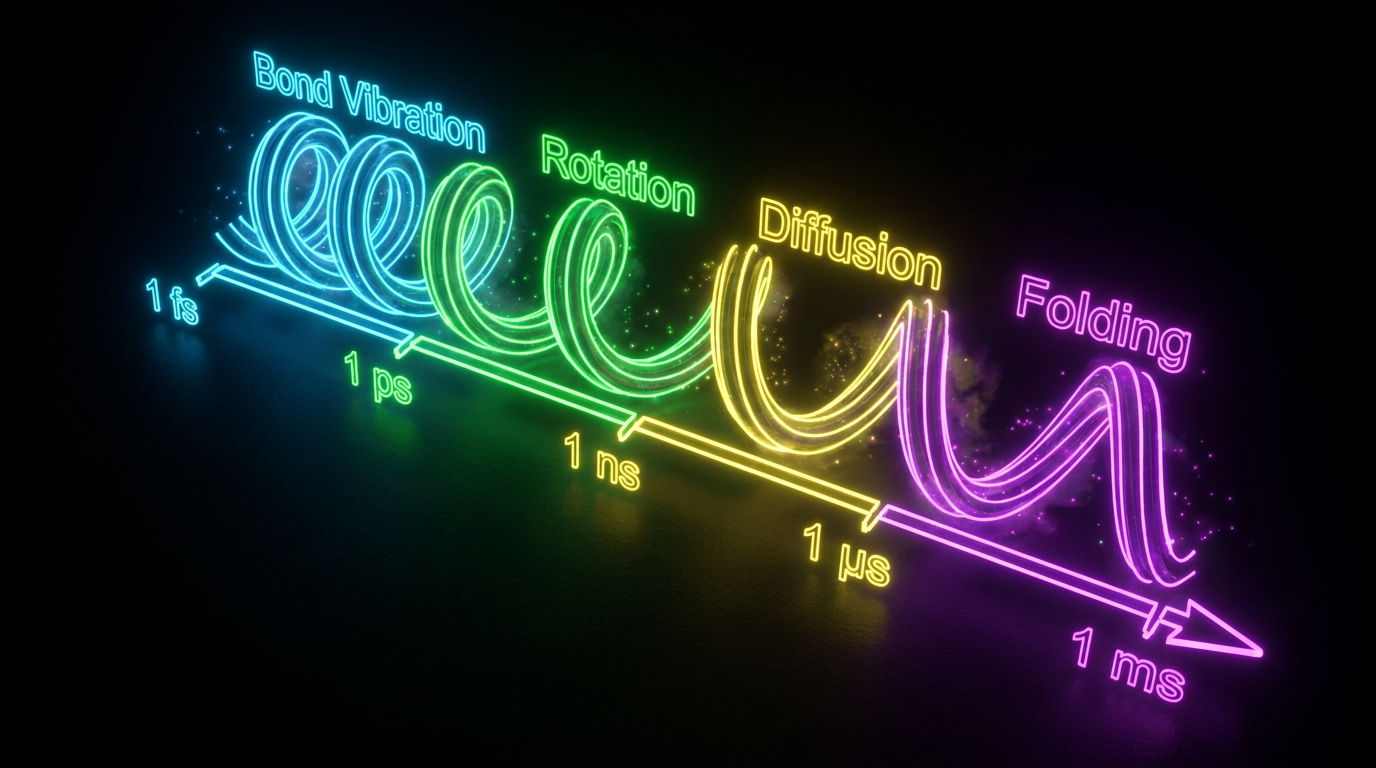
\includegraphics[width=0.85\linewidth]{assets/figures/timescale_hierarchy.png}
	\end{center}
	\begin{pitemize}
		\item \textbf{fs} \ensuremath{\rightarrow} bonds, \textbf{ps} \ensuremath{\rightarrow} water, \textbf{ns} \ensuremath{\rightarrow} sidechains, \textbf{$\mu$s} \ensuremath{\rightarrow} folding, \textbf{ms--s} \ensuremath{\rightarrow} rare
	\end{pitemize}
\end{frame}

\begin{frame}{Simulation Length --- $T = N_{\text{steps}}\times dt$}
	\begin{columns}[T,onlytextwidth]
		\column{0.5\textwidth}
		\begin{pitemize}
			\item $N_{\text{steps}} = T/dt$
			\item $100$ ns at $2$ fs \ensuremath{\rightarrow} $50$M steps
			\item Cost: $10^9$ force calls = GPU-days
		\end{pitemize}
		\column{0.5\textwidth}
		\begin{tikzpicture}[scale=1.0]
			\draw[accentcyan,thick] (0,0) rectangle (2.6,1.4);
			\foreach \y in {0.2,0.5,0.8,1.1} {\draw[softgray] (0,\y) -- (2.6,\y);}
			\node[color=fgwhite] at (1.3,1.2) {steps};
			\draw[->,thick,neonyellow] (0,-0.3) -- (2.6,-0.3) node[midway,below]{$T$};
			\draw[|<->|,accentcyan,thick] (0,1.6) -- (0.4,1.6) node[midway,above]{$dt$};
		\end{tikzpicture}
	\end{columns}
\end{frame}

\begin{frame}{Meme --- Timescales (This is Fine + Race)}
	\begin{columns}[T,onlytextwidth]
		\column{0.5\textwidth}
		\memeinclude[width=\linewidth]{assets/memes/thisisfine_meme.png}
		{\footnotesize\color{softgray} This is Fine: dt=5 fs in production}
		\column{0.5\textwidth}
		\memeinclude[width=\linewidth]{assets/memes/timescales_meme.png}
		{\footnotesize\color{softgray} Snail (ms) vs Cheetah (fs)}
	\end{columns}
\end{frame}

\begin{frame}{Interpretation --- Timescales}
	\interpret{
		\textbf{$dt$} · 1--2 fs · \textbf{hierarchy} · fs\ensuremath{\rightarrow}ms · \textbf{$T=Ndt$} · steps = cost · \textbf{rare} · need tricks · \textbf{clock} vs \textbf{biology} mismatch
	}
\end{frame}

% 06 --- Static vs Dynamic
\section{Static vs Dynamic Molecular Systems}

\begin{frame}{Static Structures --- Frozen Snapshots}
	\begin{columns}[T,onlytextwidth]
		\column{0.5\textwidth}
		\begin{pitemize}
			\item \textbf{Static}: single $\mathbf{R}$, no $T$, no motion
			\item Where you look: \textbf{crystal}, \textbf{PDB}, \textbf{DFT optimum}
			\item Question: \textit{what is stable?}
		\end{pitemize}
		\column{0.5\textwidth}
		\begin{tikzpicture}[scale=1.0]
			\shade[ball color=accentcyan] (0,0) circle (0.32cm);
			\shade[ball color=accentcyan] (1.1,0) circle (0.32cm);
			\draw[thick,white] (0,0)--(1.1,0);
			\node[color=softgray] at (0.55,-0.6) {fixed distance};
			\only<2>{\draw[dashed,neonyellow] (0,0) circle (0.5cm) node[above,color=neonyellow]{no vibration};}
		\end{tikzpicture}
	\end{columns}
\end{frame}

\subsection{Energy Minimization \& DFT}
\begin{frame}{Energy Minimization}
	\begin{equation*}
		\min_{\mathbf{R}} U(\mathbf{R}) \quad\Rightarrow\quad \mathbf{F}= -\nabla U =0,\; \text{Hessian}>0
	\end{equation*}
	\begin{columns}[T,onlytextwidth]
		\column{0.5\textwidth}
		\begin{pitemize}
			\item Steepest descent / CG / L-BFGS
			\item Finds \textbf{nearest} minimum, not global
			\item No $T$, no entropy
		\end{pitemize}
		\column{0.5\textwidth}
		\begin{tikzpicture}[scale=1.0]
			\draw[->,accentcyan] (0,0)--(2.6,0) node[right]{$R$};
			\draw[->,accentcyan] (0,0)--(0,1.6) node[above]{$U$};
			\draw[neongreen,thick,domain=0.2:2.4,samples=50] plot (\x,{1.2*exp(-(\x-0.8)*(\x-0.8)*3)+0.5*exp(-(\x-1.8)*(\x-1.8)*5)+0.2});
			\draw[->,thick,neonyellow] (0.2,1.2) -- (0.8,0.6) node[midway,above,sloped]{minimize};
			\fill[neonpink] (1.8,0.45) circle (2pt) node[below,color=neonpink]{trapped};
		\end{tikzpicture}
	\end{columns}
\end{frame}

\begin{frame}{Geometry Optimization \& DFT}
	\begin{columns}[T,onlytextwidth]
		\column{0.5\textwidth}
		\begin{pitemize}
			\item \textbf{Geom. opt.}: MM minimization (FF)
			\item \textbf{DFT}: QM minimization, \textit{ab initio} $U$
			\item Cost: DFT $\sim10^3\times$ MM
			\item Still 0 K
		\end{pitemize}
		\column{0.5\textwidth}
		\begin{infobox}[DFT $\approx$ Exact for $U$, Still Static]
			\footnotesize No temperature \ensuremath{\rightarrow} no entropy \ensuremath{\rightarrow} free energy missing
		\end{infobox}
	\end{columns}
\end{frame}

\subsection{Levinthal Paradox}
\begin{frame}{The Paradox --- Why Proteins Fold Fast}
	\begin{columns}[T,onlytextwidth]
		\column{0.55\textwidth}
		\begin{pitemize}
			\item Protein: $10^{2}$ aa, $3^{100}\sim10^{47}$ conformations
			\item Random search: $10^{27}$ yr
			\item Reality: ms--s \ensuremath{\rightarrow} \glowstrong{Levinthal paradox}
			\item Resolution: \textbf{funnel}, not flat --- downhill + guides
		\end{pitemize}
		\column{0.45\textwidth}
		\memeinclude[width=0.95\linewidth]{assets/memes/levinthal_meme.png}
	\end{columns}
\end{frame}

\begin{frame}{Funnel TikZ}
	\begin{center}
		\begin{tikzpicture}[scale=1.0]
			\shade[top color=neonyellow!30,bottom color=neonpink!60] (0,2) -- (-1.6,0) -- (1.6,0) -- cycle;
			\draw[accentcyan,thick] (-1.6,0) -- (0,2) -- (1.6,0);
			\draw[neongreen,thick,decorate,decoration={random steps,segment length=2mm,amplitude=0.6mm}] (0,1.7) -- (-0.3,0.8) -- (0.2,0.3) -- (0,0.1);
			\fill[neonpink] (0,0.1) circle (2.5pt) node[right,color=neonpink]{native};
			\node[color=softgray] at (0,2.3) {unfolded entropy};
			\node[color=bgblack] at (0,1) {funnel \ensuremath{\rightarrow} bias};
		\end{tikzpicture}
	\end{center}
\end{frame}

\subsection{Free-Energy Landscape}
\begin{frame}{Thermodynamic Stability --- $F$, Not $U$}
	\begin{equation*}
		\Delta G = \Delta H - T\Delta S \qquad p\propto e^{-\beta G}
	\end{equation*}
	\begin{pitemize}
		\item Min $U$ \ensuremath{\neq} min $F$ at $T>0$
		\item Entropy pushes to \textbf{broad} basins
		\item Solvent: \textbf{hydrophobic} = entropy of water
	\end{pitemize}
\end{frame}

\begin{frame}{Solvent Effects}
	\begin{columns}[T,onlytextwidth]
		\column{0.5\textwidth}
		\begin{pitemize}
			\item Explicit water: $10^4$ molecules, PBC
			\item Implicit: GB/SA, continuum
			\item Rigorous: solvent = \textbf{free energy}, not just screening
		\end{pitemize}
		\column{0.5\textwidth}
		\begin{tikzpicture}[scale=1.0]
			\shade[ball color=accentcyan] (0,0) circle (0.4cm) node[color=white]{solute};
			\foreach \a in {0,45,90,135,180,225,270,315} {\shade[ball color=neonblue!70] (\a:1) circle (0.18cm);}
			\node[color=neonblue] at (0,-1.5) {first shell};
		\end{tikzpicture}
	\end{columns}
\end{frame}

\begin{frame}{Interpretation --- Static vs Dynamic}
	\interpret{
		\textbf{static} · 0 K · min $U$ · \textbf{Levinthal} · $10^{47}$ vs ms · \textbf{funnel} solves · \textbf{stability} = min $F$ · \textbf{solvent} = entropy · \textbf{dynamic} = MD needed
	}
\end{frame}

% 07 --- Molecular Dynamics
\section{Molecular Dynamics}

\begin{frame}{Newton's Equations --- The Engine}
	\begin{equation*}
		m_i\ddot{\mathbf{r}}_i = \mathbf{F}_i = -\nabla_{\mathbf{r}_i}U(\mathbf{R}) \qquad \mathbf{v}_i=\dot{\mathbf{r}}_i
	\end{equation*}
	\begin{columns}[T,onlytextwidth]
		\column{0.5\textwidth}
		\begin{pitemize}
			\item $U\to$ force \ensuremath{\rightarrow} acceleration \ensuremath{\rightarrow} move
			\item Need: \textbf{positions}, \textbf{velocities}, \textbf{forces}
			\item Deterministic if $U$ exact
		\end{pitemize}
		\column{0.5\textwidth}
		\begin{tikzpicture}[scale=1.0]
			\node[draw=accentcyan,fill=darkgray,rounded corners=1mm,minimum width=2.8cm,minimum height=1.0cm,font=\footnotesize] (u) at (0,1.8) {\color{fgwhite} $U(\mathbf{R})$};
			\node[draw=neongreen,fill=darkgray,rounded corners=1mm,minimum width=2.8cm,minimum height=1.0cm,font=\footnotesize] (f) at (0,0) {\color{neongreen} $\mathbf{F}=-\nabla U$};
			\node[draw=neonyellow,fill=darkgray,rounded corners=1mm,minimum width=2.8cm,minimum height=1.0cm,font=\footnotesize] (r) at (0,-1.8) {\color{neonyellow} $\mathbf{r}(t)$};
			\draw[->,thick,accentcyan] (u) -- (f);
			\draw[->,thick,neongreen] (f) -- (r);
			\draw[->,thick,neonyellow,dashed] (r) to[bend left=40] (u) node[midway,right=10pt,font=\footnotesize]{update $U$};
		\end{tikzpicture}
	\end{columns}
\end{frame}

\subsection{Integration}
\begin{frame}{Numerical Integration --- Verlet}
	\begin{equation*}
		\mathbf{r}(t+dt)=2\mathbf{r}(t)-\mathbf{r}(t-dt)+\frac{\mathbf{F}(t)}{m}dt^2 + O(dt^4)
	\end{equation*}
	\begin{columns}[T,onlytextwidth]
		\column{0.5\textwidth}
		\begin{pitemize}
			\item \textbf{Verlet}: time-reversible, symplectic \ensuremath{\rightarrow} stable
			\item \textbf{Errors}: $O(dt^4)$ per step, $O(dt^2)$ global
			\item SHAKE/RATTLE \ensuremath{\rightarrow} constrain H-bonds \ensuremath{\rightarrow} larger $dt$
		\end{pitemize}
		\column{0.5\textwidth}
		\begin{tikzpicture}[scale=1.0]
			\draw[->,accentcyan] (0,0)--(2.6,0) node[right]{$t$};
			\foreach \x/\lab in {0.4/$t-dt$,1.3/$t$,2.2/$t+dt$} {\fill[accentcyan] (\x,0) circle (2pt) node[below]{\lab};}
			\draw[<->,thick,neonyellow] (0.4,0.5)--(1.3,0.5) node[midway,above]{$dt$};
			\only<2>{\node[color=neonpink] at (1.3,1) {no velocities needed!};}
		\end{tikzpicture}
	\end{columns}
\end{frame}

\subsection{Workflow}
\begin{frame}{MD Workflow --- From $\mathbf{r}_0$ to Trajectory}
	\begin{center}
		\begin{tikzpicture}[scale=1.0]
			\foreach \idx/\txt in {0/{$\mathbf{r}_0,\mathbf{v}_0$},1/Forces,2/Integrate,3/Trajectory} {
			\node[draw=accentcyan,rounded corners=2mm,fill=darkgray,minimum width=2.6cm,minimum height=1.0cm,align=center,font=\footnotesize] (n\idx) at (\idx*3.2,0) {\color{fgwhite} \txt};
			}
			\draw[->,thick,accentcyan] (n0) -- (n1);
			\draw[->,thick,accentcyan] (n1) -- (n2);
			\draw[->,thick,accentcyan] (n2) -- (n3);
			\node[draw=neonyellow,fill=neonyellow!15,rounded corners=1mm,inner sep=1.5mm,font=\footnotesize] at (1.6,1.2) {IC: Maxwell--Boltzmann};
			\node[draw=neongreen,fill=neongreen!15,rounded corners=1mm,inner sep=1.5mm,font=\footnotesize] at (4.8,1.2) {Equil. \ensuremath{\rightarrow} Prod.};
		\end{tikzpicture}
	\end{center}
	\begin{pitemize}
		\item \textbf{Initial conditions}: positions (PDB) + velocities ($\propto\sqrt{T}$)
		\item \textbf{Equilibration}: relax $T,P$, density plateau
		\item \textbf{Production}: N steps \ensuremath{\rightarrow} \textbf{trajectory} + \textbf{sampling}
	\end{pitemize}
\end{frame}

\begin{frame}{Convergence --- When to Stop?}
	\begin{columns}[T,onlytextwidth]
		\column{0.5\textwidth}
		\begin{pitemize}
			\item \textbf{Convergence}: $\langle A\rangle$ stops drifting
			\item Check: $\langle T\rangle$, RMSD plateau, block error
			\item \textbf{Longer} \ensuremath{\neq} \textbf{converged} if $\tau$ huge
		\end{pitemize}
		\column{0.5\textwidth}
		\begin{tikzpicture}[scale=1.0]
			\draw[->,accentcyan] (0,0)--(2.6,0) node[right]{$t$};
			\draw[->,accentcyan] (0,0)--(0,1.6) node[above]{$\langle A\rangle$};
			\draw[neongreen,thick,domain=0:2.4,samples=40] plot (\x,{0.4+0.6*exp(-\x*1.5)+0.2*sin(\x*10 r)*exp(-\x*0.5)});
			\draw[dashed,neonyellow] (0,0.4) -- (2.4,0.4) node[right,color=neonyellow]{limit};
		\end{tikzpicture}
	\end{columns}
\end{frame}

\begin{frame}{Meme --- Pikachu Surprise}
	\begin{center}
		\memeinclude[width=0.7\linewidth]{assets/memes/pikachu_meme.png}
		{\footnotesize\color{softgray} When dt=5 fs and system explodes --- \textit{surprised}}
	\end{center}
\end{frame}

\begin{frame}{Interpretation --- MD}
	\interpret{
		\textbf{Newton} · $F=-\nabla U$ · \textbf{Verlet} · reversible · \textbf{IC} · Maxwell · \textbf{trajectory} · equil.\ensuremath{\rightarrow}prod. · \textbf{convergence} · plateau · \textbf{sampling} = statistics
	}
\end{frame}

% 08 --- Simulation Data Analysis
\section{Simulation Data Analysis}

\begin{frame}{Trajectory --- The Movie}
	\begin{columns}[T,onlytextwidth]
		\column{0.5\textwidth}
		\begin{pitemize}
			\item \textbf{Trajectory}: $\{\mathbf{R}(t_0),\mathbf{R}(t_1),\dots\}$ --- DCD/XTC
			\item Size: $N\times 3\times N_{\text{frames}}\times 4$ bytes
			\item \textbf{Analysis} = compress movie \ensuremath{\rightarrow} numbers
		\end{pitemize}
		\column{0.5\textwidth}
		\begin{center}
			\begin{tikzpicture}[scale=1.0]
				% Three snapshot frames showing molecule moving
				\foreach \idx/\dx/\dy in {0/0/0.2,1/2.2/0.0,2/4.4/-0.15} {
						\draw[accentcyan,thick,rounded corners=1mm,fill=darkgray] (\idx*2.0,0) rectangle ++(1.6,1.4);
						\shade[ball color=neonblue] (\idx*2.0+0.5,0.7+\dy) circle (0.12);
						\shade[ball color=neonpink] (\idx*2.0+1.0,0.5+\dy) circle (0.10);
						\shade[ball color=neongreen] (\idx*2.0+0.8,1.0+\dy) circle (0.09);
					}
				% Arrows between frames
				\draw[->,thick,neonyellow] (1.6,0.7) -- (2.0,0.7);
				\draw[->,thick,neonyellow] (3.6,0.7) -- (4.0,0.7);
				\node[color=softgray,font=\footnotesize] at (2.8,-0.3) {$t_0 \to t_1 \to t_2$};
				\node[color=accentcyan,font=\footnotesize] at (0.8,1.7) {frame 0};
				\node[color=accentcyan,font=\footnotesize] at (2.8,1.7) {frame 1};
				\node[color=accentcyan,font=\footnotesize] at (4.8,1.7) {frame 2};
			\end{tikzpicture}
		\end{center}
	\end{columns}
\end{frame}

\subsection{Geometric Measures}
\begin{frame}{RMSD, RMSF, $R_g$}
	\begin{columns}[T,onlytextwidth]
		\column{0.33\textwidth}
		\begin{infobox}[RMSD]
			\footnotesize $\text{RMSD}(t)=\sqrt{\frac1N\sum_i |\mathbf{r}_i(t)-\mathbf{r}_i^{\text{ref}}|^2}$\\\footnotesize drift = motion
		\end{infobox}
		\column{0.33\textwidth}
		\begin{infobox}[RMSF]
			\footnotesize $\text{RMSF}_i=\sqrt{\langle (\mathbf{r}_i-\langle\mathbf{r}_i\rangle)^2\rangle}$\\\footnotesize flexibility per residue
		\end{infobox}
		\column{0.33\textwidth}
		\begin{infobox}[R$_g$]
			\footnotesize $R_g^2=\frac1N\sum_i |\mathbf{r}_i-\mathbf{r}_{\text{COM}}|^2$\\\footnotesize compactness
		\end{infobox}
	\end{columns}
\end{frame}

\begin{frame}{H-Bonds, Distances, Angles}
	\begin{columns}[T,onlytextwidth]
		\column{0.5\textwidth}
		\begin{pitemize}
			\item \textbf{H-bond}: $d_{\text{O}\cdots\text{H}}<3.5$Å, $\angle>150^\circ$
			\item Distances/angles \ensuremath{\rightarrow} \textbf{order parameters}
			\item \textbf{Define} before measuring
		\end{pitemize}
		\column{0.5\textwidth}
		\begin{tikzpicture}[scale=1.0]
			\shade[ball color=neonblue] (0,0) circle (0.32cm) node[color=white]{O};
			\shade[ball color=neonyellow] (1,0.6) circle (0.22cm) node[color=bgblack]{H};
			\draw[dashed,neonpink,thick] (0,0) -- (1,0.6) node[midway,above,sloped]{H-bond};
			\draw[accentcyan,thick] (1,0.6) -- (2,0.2);
			\draw[neonyellow] (1,0.6) -- (1.5,0.3) arc (30:-10:0.4cm);
			\node[color=neonyellow] at (1.6,0.2) {$\theta$};
		\end{tikzpicture}
	\end{columns}
\end{frame}

\subsection{RDF \& Clustering}
\begin{frame}{Radial Distribution Function}
	\begin{equation*}
		g(r)=\frac{\langle \rho(r)\rangle}{\rho_0} \quad\text{--- shell structure}
	\end{equation*}
	\begin{columns}[T,onlytextwidth]
		\column{0.5\textwidth}
		\begin{pitemize}
			\item First peak \ensuremath{\rightarrow} coordination shell
			\item $g(r)\to1$ at long $r$
			\item Integrates to $n(r)=4\pi\rho_0\int_0^r g(s)s^2ds$
		\end{pitemize}
		\column{0.5\textwidth}
		\begin{tikzpicture}[scale=1.0]
			\draw[->,accentcyan] (0,0)--(2.6,0) node[right]{$r$};
			\draw[->,accentcyan] (0,0)--(0,1.6) node[above]{$g(r)$};
			\draw[neongreen,thick] plot[smooth] coordinates {(0.3,0.2) (0.5,1.0) (0.7,1.4) (0.9,0.8) (1.1,0.5) (1.3,0.7) (1.5,0.55) (1.7,0.52) (1.9,0.51) (2.1,0.5) (2.4,0.5)};
			\draw[dashed,softgray] (0,1) -- (2.4,1) node[right,color=softgray]{1};
			\node[color=neongreen] at (0.7,1.4) {1st shell};
		\end{tikzpicture}
	\end{columns}
\end{frame}

\begin{frame}{Conformational Clustering}
	\begin{columns}[T,onlytextwidth]
		\column{0.5\textwidth}
		\begin{pitemize}
			\item Group frames by RMSD \ensuremath{\rightarrow} \textbf{clusters}
			\item Representative = medoid
			\item \textbf{Why?} \ensuremath{\rightarrow} reduce $10^6$ frames \ensuremath{\rightarrow} 5 states
		\end{pitemize}
		\column{0.5\textwidth}
		\begin{center}
			\begin{tikzpicture}[scale=1.1]
				% Cluster 1 (pink, top-left)
				\draw[neonpink,dashed,thick,rounded corners=3mm] (-0.1,-0.1) rectangle (1.3,1.3);
				\fill[neonpink] (0.3,0.4) circle (3pt);
				\fill[neonpink] (0.6,0.7) circle (3pt);
				\fill[neonpink] (0.4,0.9) circle (3pt);
				\fill[neonpink] (0.9,0.3) circle (3pt);
				\node[color=neonpink,font=\footnotesize\bfseries] at (0.6,1.55) {C1};
				% Cluster 2 (green, top-right)
				\draw[neongreen,dashed,thick,rounded corners=3mm] (1.8,0.1) rectangle (3.2,1.3);
				\fill[neongreen] (2.1,0.6) circle (3pt);
				\fill[neongreen] (2.5,0.4) circle (3pt);
				\fill[neongreen] (2.8,0.9) circle (3pt);
				\fill[neongreen] (2.3,1.0) circle (3pt);
				\node[color=neongreen,font=\footnotesize\bfseries] at (2.5,1.55) {C2};
				% Cluster 3 (yellow, bottom)
				\draw[neonyellow,dashed,thick,rounded corners=3mm] (0.8,-1.3) rectangle (2.4,-0.1);
				\fill[neonyellow] (1.2,-0.5) circle (3pt);
				\fill[neonyellow] (1.6,-0.8) circle (3pt);
				\fill[neonyellow] (2.0,-0.4) circle (3pt);
				\node[color=neonyellow,font=\footnotesize\bfseries] at (1.6,-1.55) {C3};
				% Medoid markers (star shape using TikZ)
				\node[color=neonpink,font=\footnotesize] at (0.6,0.7) {$\star$};
				\node[color=neongreen,font=\footnotesize] at (2.5,0.6) {$\star$};
				\node[color=neonyellow,font=\footnotesize] at (1.6,-0.6) {$\star$};
			\end{tikzpicture}
		\end{center}
	\end{columns}
\end{frame}

\subsection{Visualization \& Titan}
\begin{frame}{Visualization --- See Before You Believe}
	\begin{columns}[T,onlytextwidth]
		\column{0.5\textwidth}
		\begin{pitemize}
			\item \textbf{VMD/PyMOL/OVITO/ChimeraX} \ensuremath{\rightarrow} see artefacts
			\item Color by \textbf{velocity}, \textbf{charge}, time
			\item \textbf{Titan} anecdote: 18,000 GPUs, 1 $\mu$s/day \ensuremath{\rightarrow} still \textbf{need} analysis
		\end{pitemize}
		\column{0.5\textwidth}
		\begin{center}
			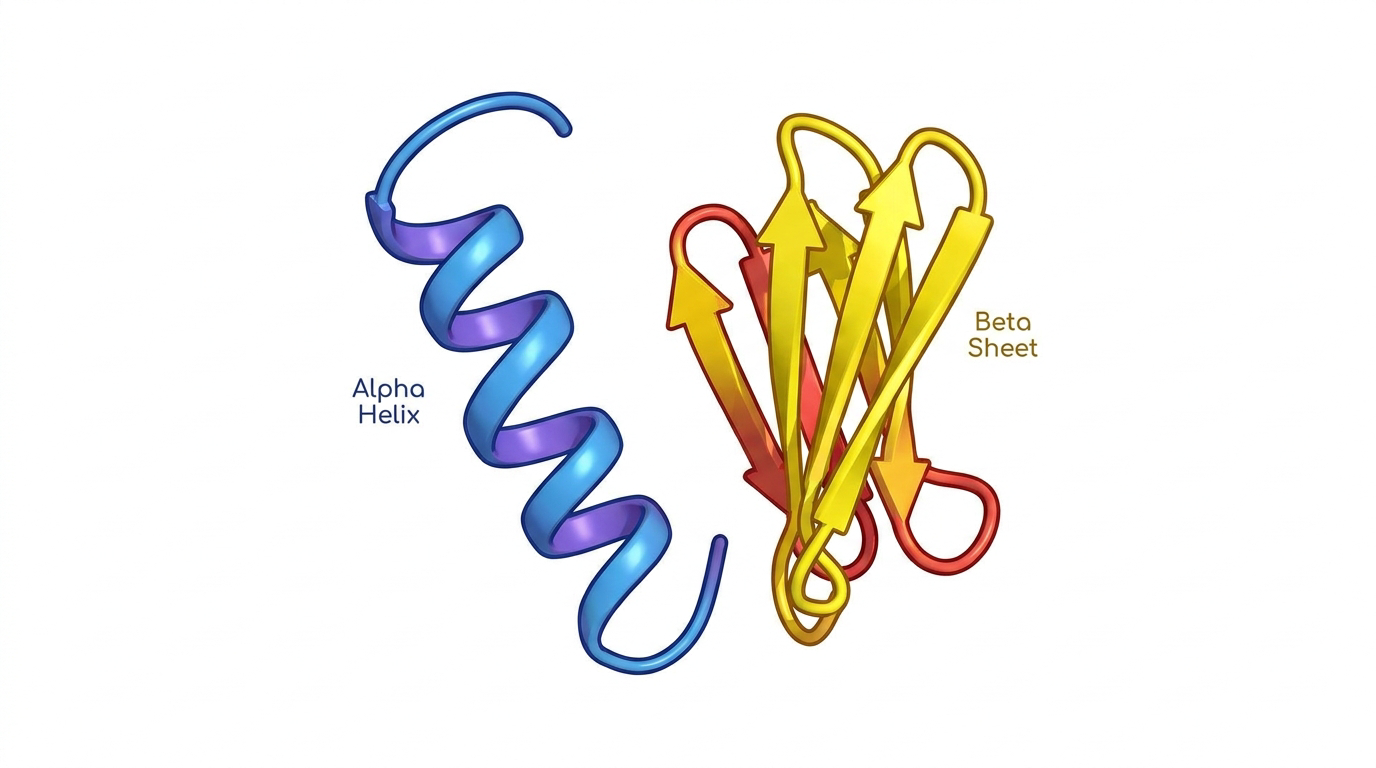
\includegraphics[width=0.9\linewidth]{assets/figures/protein_cartoon.png}
			{\footnotesize\color{softgray} PyMOL-style cartoon: helices + sheets}
		\end{center}
	\end{columns}
\end{frame}

\begin{frame}{LJ Fluid --- What Your Trajectory Looks Like}
	\begin{center}
		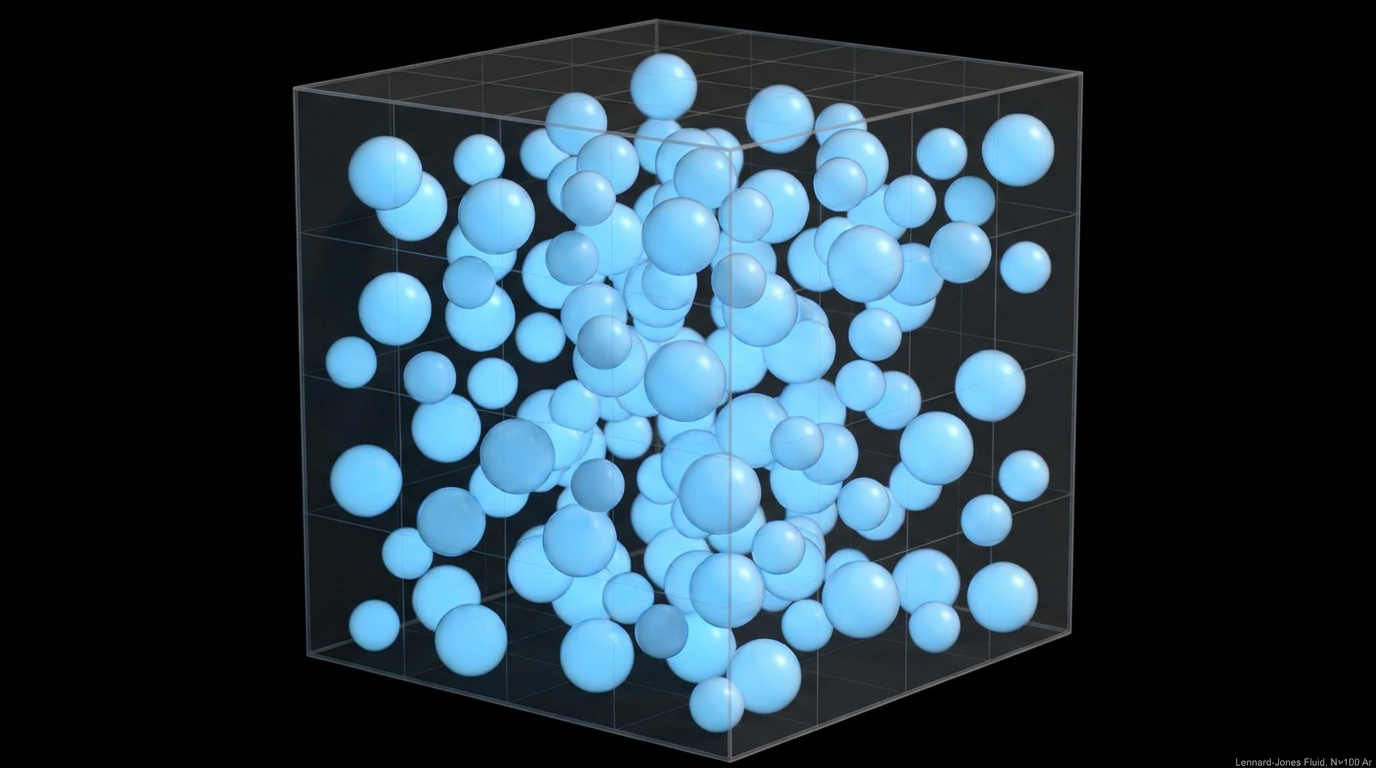
\includegraphics[width=0.7\linewidth]{assets/figures/lj_fluid_snapshot.png}
		{\footnotesize\color{softgray} Lennard-Jones fluid snapshot (OVITO view)}
	\end{center}
\end{frame}

\begin{frame}{Interpretation --- Analysis}
	\interpret{
		\textbf{trajectory} · movie · \textbf{RMSD} · drift · \textbf{RMSF} · flex · \textbf{$R_g$} · compact · \textbf{H-bond} · geometry · \textbf{$g(r)$} · shells · \textbf{clustering} · 5 states · \textbf{visualize} · trust
	}
\end{frame}

% 09 --- Enhanced Sampling
\section{Enhanced Sampling and Free-Energy Methods}

\begin{frame}{The Sampling Problem}
	\begin{columns}[T,onlytextwidth]
		\column{0.5\textwidth}
		\begin{pitemize}
			\item MD samples $\propto e^{-\beta U}$ \ensuremath{\rightarrow} rare events \textbf{never} seen
			\item Barrier $10\,k_BT$ \ensuremath{\rightarrow} wait $e^{10}\sim 20$k× longer
			\item \textbf{Biology lives in rare events}
		\end{pitemize}
		\column{0.5\textwidth}
		\begin{center}
			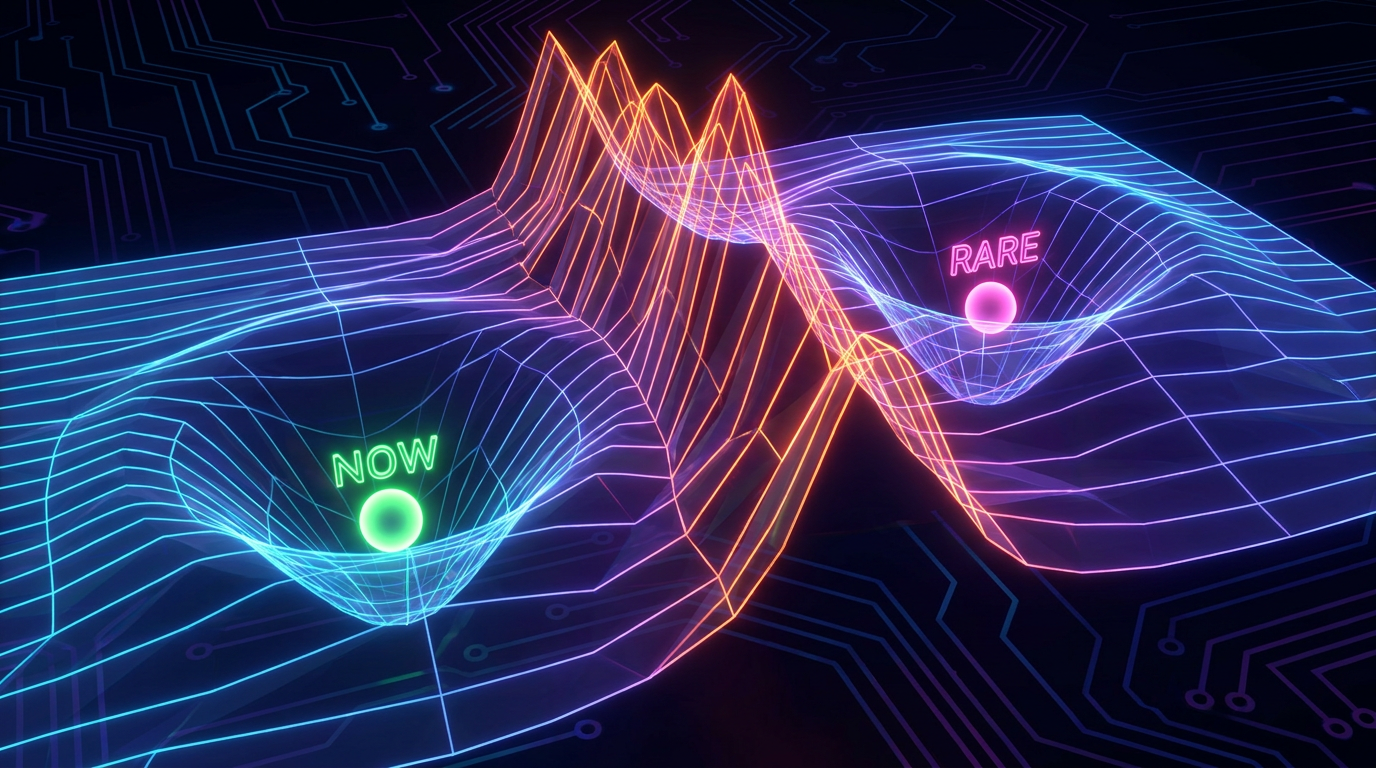
\includegraphics[width=0.9\linewidth]{assets/figures/sampling_barrier.png}
			{\footnotesize\color{softgray} MD stuck in left well, rare event in right}
		\end{center}
	\end{columns}
\end{frame}

\subsection{Methods}
\begin{frame}{Metadynamics --- Fill the Well}
	\begin{equation*}
		V_{\text{bias}}(s,t)=\sum_{t'} w\, e^{-(s-s(t'))^2/2\sigma^2}
	\end{equation*}
	\begin{columns}[T,onlytextwidth]
		\column{0.5\textwidth}
		\begin{pitemize}
			\item Deposit Gaussians along CV $s$
			\item Flood minima \ensuremath{\rightarrow} escape
			\item \textbf{Free energy} = $-V_{\text{bias}}$ at convergence
		\end{pitemize}
		\column{0.5\textwidth}
		\begin{tikzpicture}[scale=1.0]
			\draw[->,accentcyan] (0,0)--(2.6,0) node[right]{$s$};
			\draw[->,accentcyan] (0,0)--(0,1.6) node[above]{$F$};
			\only<1>{\draw[neongreen,thick] plot[smooth] coordinates {(0.2,0.3) (0.5,1.0) (0.8,1.1) (1.0,0.5) (1.3,0.4) (1.6,0.9) (1.8,1.1) (2.1,0.5) (2.4,0.3)};}
			\only<2>{\draw[neonyellow,thick] plot[smooth] coordinates {(0.2,0.3) (0.5,0.4) (0.8,0.45) (1.0,0.4) (1.3,0.38) (1.6,0.42) (1.8,0.45) (2.1,0.4) (2.4,0.3)}; \node[color=neonyellow] at (1.3,1.3) {filled};}
		\end{tikzpicture}
	\end{columns}
\end{frame}

\begin{frame}{Umbrella Sampling --- Windows}
	\begin{columns}[T,onlytextwidth]
		\column{0.5\textwidth}
		\begin{pitemize}
			\item Harmonic umbrella per window: $w_i(s)=\tfrac12k(s-s_i)^2$
			\item Overlap windows \ensuremath{\rightarrow} WHAM/MBAR
			\item Rigorous $PMF$ via reweighting
		\end{pitemize}
		\column{0.5\textwidth}
		\begin{tikzpicture}[scale=1.0]
			\draw[->,accentcyan] (0,0)--(2.8,0) node[right]{$s$};
			\foreach \x in {0.5,1.2,1.9} {\draw[neongreen,thick] plot[smooth] coordinates {(\x-0.3,0.2) (\x-0.15,0.5) (\x,1.0) (\x+0.15,0.5) (\x+0.3,0.2)}; \fill[accentcyan] (\x,0.2) circle (1.5pt);}
			\node[color=softgray] at (1.4,-0.3) {windows + umbrellas};
		\end{tikzpicture}
	\end{columns}
\end{frame}

\begin{frame}{Replica Exchange \& Accelerated MD}
	\begin{columns}[T,onlytextwidth]
		\column{0.5\textwidth}
		\begin{pitemize}
			\item \textbf{Replica exchange}: hot replicas \ensuremath{\rightarrow} cold via swap $P\propto e^{\Delta\beta\Delta U}$
			\item \textbf{Accelerated MD}: boost $U \to U+\Delta V$ when $U<$ threshold
		\end{pitemize}
		\column{0.5\textwidth}
		\begin{tikzpicture}[scale=1.0]
			\foreach \y in {0,0.7,1.4} {
					\draw[accentcyan] (0,\y) -- (2.2,\y);
					\foreach \x in {0.3,0.9,1.5,2.0} {\fill[neongreen] (\x,\y) circle (1pt);}
				}
			\draw[<->,thick,neonyellow] (2.4,0) -- (2.4,1.4) node[midway,right]{$T$};
			\draw[dashed,neonpink] (0.9,0) -- (0.9,1.4);
		\end{tikzpicture}
	\end{columns}
\end{frame}

\begin{frame}{Potential of Mean Force}
	\begin{equation*}
		W(s) = -k_BT\ln P(s) \qquad P(s)=\langle\delta(s-s(\mathbf{R}))\rangle
	\end{equation*}
	\begin{pitemize}
		\item PMF = free energy \textbf{along} CV
		\item Minimum = stable, barrier = rate via Kramers
	\end{pitemize}
\end{frame}

\begin{frame}{Interpretation --- Enhanced Sampling}
	\interpret{
		\textbf{rare} · barrier wins · \textbf{metadynamics} · fill wells · \textbf{umbrella} · windows \ensuremath{\rightarrow} WHAM · \textbf{replica} · heat helps · \textbf{PMF} · $ -kT\ln P$ · \textbf{free energy} = truth
	}
\end{frame}

% 10 --- Molecular Simulation Software
\section{Molecular Simulation Software}

\begin{frame}{Ecosystem --- Who Does What}
  \begin{center}
    \begin{tikzpicture}[scale=0.9]
      \foreach \idx/\eng/\col in {0/LAMMPS/accentcyan,1/GROMACS/neongreen,2/OpenMM/neonyellow,3/NAMD/neonpink,4/AMBER/neonblue,5/CHARMM/customblue} {
        \node[draw=\col,fill=darkgray,rounded corners=1.5mm,minimum width=1.8cm,minimum height=0.6cm,align=center] at (\idx*2.0,0.8) {\color{fgwhite}\tiny \eng};
      }
      \foreach \idx/\tool/\col in {0/VMD/accentcyan,1/PyMOL/neongreen,2/OVITO/neonyellow,3/ChimeraX/neonpink} {
        \node[draw=\col,fill=darkgray,rounded corners=1.5mm,minimum width=1.8cm,minimum height=0.6cm,align=center] at (\idx*2.0+1, -0.4) {\color{fgwhite}\tiny \tool};
      }
      \node[color=softgray] at (5,0.8) {engines};
      \node[color=softgray] at (5,-0.4) {viewers};
    \end{tikzpicture}
  \end{center}
  \begin{pitemize}
    \item \textbf{LAMMPS}: materials, all-atom, coarse-grained, \textbf{you built it}
    \item \textbf{GROMACS}: biomolecules, fast, PME
    \item \textbf{OpenMM}: GPU, Python API, custom forces
  \end{pitemize}
\end{frame}

\begin{frame}{Choosing --- Cheat Sheet}
  \begin{columns}[T,onlytextwidth]
    \column{0.5\textwidth}
    \begin{infobox}[Pick by System]
      \scriptsize Metals/polymers \ensuremath{\rightarrow} LAMMPS\\ Biomembrane/protein \ensuremath{\rightarrow} GROMACS/AMBER\\ Custom \ensuremath{\rightarrow} OpenMM\\ Visualize \ensuremath{\rightarrow} VMD/OVITO
    \end{infobox}
    \column{0.5\textwidth}
    \begin{warningbox}[All Need]
      \scriptsize Force field \textbf+++ \textbf{PBC} + \textbf{thermostat} + \textbf{analysis}
    \end{warningbox}
  \end{columns}
\end{frame}

\begin{frame}{Meme --- Distracted Simulator}
  \begin{center}
    \memeinclude[width=0.7\linewidth]{assets/memes/distracted_meme.png}
    {\scriptsize\color{softgray} Distracted Boyfriend: Simulator \ensuremath{\rightarrow} ML potentials (goodbye Classical FF)}
  \end{center}
\end{frame}

\begin{frame}{Interpretation --- Software}
  \interpret{
    \textbf{LAMMPS} · materials · \textbf{GROMACS} · bio · \textbf{OpenMM} · GPU Python · \textbf{VMD/OVITO} · eyes · \textbf{all} · $U$+PBC+sampling
  }
\end{frame}

% 11 --- Hands-on LAMMPS
\section{Hands-on LAMMPS Simulation}

\begin{frame}[fragile]{Installation --- One Script, Both OS}
  \begin{columns}[T,onlytextwidth]
    \column{0.5\textwidth}
    \begin{minted}[fontsize=\tiny,bgcolor=codebg]{bash}
# Linux ( Xeons 24c + A100 sm_80 )
./scripts/build-lammps.sh   # most+gpu+kokkos
# Windows PowerShell
.\scripts\build-lammps.ps1
# Check
./lammps/build/lmp -h | head
    \end{minted}
    \column{0.5\textwidth}
    \begin{successbox}[You Built 65 Packages]
      \scriptsize \texttt{lmp -h} shows GPU (mixed, sm\_80) + KOKKOS (CUDA, AMPERE80) + 24 cores
    \end{successbox}
  \end{columns}
\end{frame}

\begin{frame}[fragile]{Input Script --- The Recipe}
  \begin{columns}[T,onlytextwidth]
    \column{0.5\textwidth}
    \begin{minted}[fontsize=\tiny,bgcolor=codebg]{text}
units real
atom_style full
read\_data water.data
pair\_style lj/cut/coul/long 10
kspace_style pppm 1e-4
fix 1 all nvt temp 300 300 100
timestep 2.0
run 50000
    \end{minted}
    \column{0.5\textwidth}
    \begin{pitemize}
      \item \textbf{Box}: \inlinecode{region + create\_box} or \inlinecode{read\_data}
      \item \textbf{Atoms}: \inlinecode{create\_atoms} or file
      \item \textbf{FF}: \inlinecode{pair\_style / bond\_style}
      \item \textbf{BC}: \inlinecode{boundary p p p}
      \item \textbf{dt}: 1--2 fs
    \end{pitemize}
  \end{columns}
\end{frame}

\begin{frame}{Execution --- Log, Trajectory, Analysis}
  \begin{columns}[T,onlytextwidth]
    \column{0.4\textwidth}
    \begin{pitemize}
      \item \inlinecode{lmp -in in.lj -log log.lammps}
      \item \textbf{Log}: thermo (step, $T$, $E$, $P$)
      \item \textbf{Trajectory}: dump \texttt{custom}/\texttt{xtc} \ensuremath{\rightarrow} VMD/OVITO
      \item \textbf{Analysis}: \texttt{compute rdf}, Python post
    \end{pitemize}
    \column{0.6\textwidth}
    \begin{tikzpicture}[scale=0.6]
      \node[draw=accentcyan,fill=darkgray,rounded corners=1mm,minimum width=2.2cm,minimum height=0.6cm] (a) at (0,0) {\color{fgwhite}\tiny in.lj};
      \node[draw=neongreen,fill=darkgray,rounded corners=1mm,minimum width=1.1cm,minimum height=0.6cm] (b) at (2.4,0.6) {\color{neongreen}\tiny log};
      \node[draw=neonyellow,fill=darkgray,rounded corners=1mm,minimum width=1.4cm,minimum height=0.6cm] (c) at (2.4,-0.6) {\color{neonyellow}\tiny dump.*};
      \draw[->,thick,accentcyan] (a) -- (1.2,0) |- (b);
      \draw[->,thick,accentcyan] (a) -- (1.2,0) |- (c);
    \end{tikzpicture}
  \end{columns}
\end{frame}

\begin{frame}{Interpretation --- LAMMPS}
  \interpret{
    \textbf{install} · \texttt{build-lammps.sh} · \textbf{script} · 5 lines \ensuremath{\rightarrow} run · \textbf{log} · $T,E,P$ · \textbf{dump} · movie · \textbf{analysis} · your science
  }
\end{frame}

% 12 --- GROMACS
\section{Introduction to GROMACS}

\begin{frame}[fragile]{Installation \& Files}
  \begin{columns}[T,onlytextwidth]
    \column{0.5\textwidth}
    \begin{minted}[fontsize=\tiny,bgcolor=codebg]{bash}
# Install (conda / apt)
conda install -c conda-forge gromacs
# Inputs
gmx pdb2gmx -f protein.pdb
gmx editconf -f conf.gro -o box.gro -c -d 1.0 -bt cubic
gmx solvate -cp box.gro -o solv.gro
    \end{minted}
    \column{0.5\textwidth}
    \begin{pitemize}
      \item \textbf{Structure}: \texttt{.gro/.pdb}
      \item \textbf{Topology}: \texttt{topol.top} (FF + bonds)
      \item \textbf{Parameters}: \texttt{.mdp} (dt, $T$, $P$)
    \end{pitemize}
  \end{columns}
\end{frame}

\begin{frame}[fragile]{GROMACS Workflow --- Min \ensuremath{\rightarrow} NVT \ensuremath{\rightarrow} NPT \ensuremath{\rightarrow} Prod}
  \begin{center}
    \begin{tikzpicture}[scale=0.9]
      \foreach \idx/\txt in {0/Minimize,1/NVT,2/NPT,3/Production} {
        \node[draw=accentcyan,rounded corners=2mm,fill=darkgray,minimum width=2.3cm,minimum height=0.7cm,align=center] (n\idx) at (\idx*2.9,0) {\color{fgwhite}\tiny \txt};
      }
      \draw[->,thick,accentcyan] (n0) -- (n1);
      \draw[->,thick,accentcyan] (n1) -- (n2);
      \draw[->,thick,accentcyan] (n2) -- (n3);
      \node[color=softgray] at (1.45,1) {\texttt{em.mdp} \ensuremath{\rightarrow} \texttt{nvt.mdp} \ensuremath{\rightarrow} \texttt{npt.mdp} \ensuremath{\rightarrow} \texttt{md.mdp}};
    \end{tikzpicture}
  \end{center}
  \begin{pitemize}
    \item \textbf{EM}: $\min U$, $F_{\max}<1000$ kJ/mol/nm
    \item \textbf{NVT}: V-rescale thermostat, $dt=2$ fs, LINCS
    \item \textbf{NPT}: Parrinello-Rahman, $P=1$ bar
    \item \textbf{Prod}: $50$ ns \ensuremath{\rightarrow} \texttt{traj.xtc} + \texttt{ener.edr}
  \end{pitemize}
\end{frame}

\begin{frame}[fragile]{Trajectory Analysis}
  \begin{minted}[fontsize=\tiny,bgcolor=codebg]{bash}
gmx rms -s topol.tpr -f traj.xtc -o rmsd.xvg
gmx gyrate -s topol.tpr -f traj.xtc -o rg.xvg
gmx rdf -s topol.tpr -f traj.xtc -o rdf.xvg
  \end{minted}
  \begin{pitemize}
    \item Same as LAMMPS: RMSD, $R_g$, $g(r)$, H-bonds
    \item Different file names, same physics
  \end{pitemize}
\end{frame}

\begin{frame}{Interpretation --- GROMACS}
  \interpret{
    \textbf{GROMACS} · bio focus · \textbf{files} · gro/top/mdp · \textbf{workflow} · min\ensuremath{\rightarrow}NVT\ensuremath{\rightarrow}NPT\ensuremath{\rightarrow}prod · \textbf{analysis} · same $g(r)$, RMSD · \textbf{PMEs} = fast Coulomb
  }
\end{frame}

% 13 --- Programming for Molecular Simulation
\section{Programming for Molecular Simulation}

\begin{frame}[fragile]{Linux \& Bash --- Your Lab Bench}
  \begin{columns}[T,onlytextwidth]
    \column{0.5\textwidth}
    \begin{minted}[fontsize=\tiny,bgcolor=codebg]{bash}
for d in */; do
  mpirun -np 24 lmp -in in.lj
  python analyse.py traj.xtc
done
    \end{minted}
    \column{0.5\textwidth}
    \begin{pitemize}
      \item \textbf{Linux}: HPC speaks bash
      \item \textbf{Automation}: loops, slurm, `snakemake`
      \item \textbf{Reproducible}: script beats clicking
    \end{pitemize}
  \end{columns}
\end{frame}

\begin{frame}[fragile]{Python Stack --- NumPy \ensuremath{\rightarrow} MDAnalysis}
  \begin{columns}[T,onlytextwidth]
    \column{0.5\textwidth}
    \begin{pitemize}
      \item \textbf{NumPy/SciPy}: arrays, FFT, linalg
      \item \textbf{Matplotlib/Pandas}: plots, tables
      \item \textbf{MDAnalysis/MDTraj}: read traj \ensuremath{\rightarrow} compute $g(r)$
      \item \textbf{RDKit}: cheminformatics
    \end{pitemize}
    \column{0.5\textwidth}
    \begin{minted}[fontsize=\tiny,bgcolor=codebg]{python}
import MDAnalysis as mda
import numpy as np
u = mda.Universe("topol.tpr","traj.xtc")
for ts in u.trajectory:
    pos = u.atoms.positions
    # compute RDF, RMSD, ...
    \end{minted}
  \end{columns}
\end{frame}

\begin{frame}{C/C++/Fortran/CUDA --- Speed}
  \begin{columns}[T,onlytextwidth]
    \column{0.5\textwidth}
    \begin{pitemize}
      \item LAMMPS/GROMACS = \textbf{C++}/CUDA/Fortran
      \item You: Python for glue, \textbf{CUDA} for custom kernels
      \item \inlinecode{uv} \ensuremath{\rightarrow} C++ \ensuremath{\rightarrow} LAMMPS plugin
    \end{pitemize}
    \column{0.5\textwidth}
    \begin{tikzpicture}[scale=0.9]
      \draw[->,accentcyan,thick] (0,0)--(2.6,0) node[right]{speed};
      \draw[->,accentcyan,thick] (0,0)--(0,1.8) node[above]{ease};
      \fill[neonyellow] (0.5,1.5) circle (3pt) node[above]{Python};
      \fill[neonpink] (2.2,0.3) circle (3pt) node[below]{CUDA};
      \fill[accentcyan] (1.4,0.9) circle (3pt) node[above]{C++};
    \end{tikzpicture}
  \end{columns}
\end{frame}

\begin{frame}{Interpretation --- Programming}
  \interpret{
    \textbf{Bash} · loop it · \textbf{Python} · NumPy/MDAnalysis · \textbf{C++/CUDA} · speed · \textbf{automation} · snakemake · \textbf{repro} = script
  }
\end{frame}

% 14 --- AI and Molecular Structure Prediction
\section{AI and Molecular Structure Prediction}

\begin{frame}{AlphaFold / OpenFold --- Sequence \ensuremath{\rightarrow} Structure}
  \begin{columns}[T,onlytextwidth]
    \column{0.5\textwidth}
    \begin{pitemize}
      \item Input: \textbf{sequence} \ensuremath{\rightarrow} Output: \textbf{3D coordinates}
      \item Attention over MSA \ensuremath{\rightarrow} distances \ensuremath{\rightarrow} structure module
      \item \textbf{Accuracy}: CASP, $ \text{lDDT} > 90$ for many
      \item \textbf{OpenFold} = open AlphaFold2
    \end{pitemize}
    \column{0.5\textwidth}
    \begin{tikzpicture}[scale=1.0]
      \node[draw=accentcyan,fill=darkgray,rounded corners=1mm,minimum width=2.2cm,minimum height=0.6cm] (s) at (0,1) {\color{fgwhite}\footnotesize SEQUENCE};
      \node[draw=neonyellow,fill=darkgray,rounded corners=1mm,minimum width=2.2cm,minimum height=0.6cm] (a) at (0,0) {\color{neonyellow}\footnotesize evo attention};
      \node[draw=neongreen,fill=darkgray,rounded corners=1mm,minimum width=2.2cm,minimum height=0.6cm] (p) at (0,-1) {\color{neongreen}\footnotesize STRUCTURE};
      \draw[->,thick,accentcyan] (s)--(a); \draw[->,thick,neonyellow] (a)--(p);
      \node[color=softgray] at (2,0) {MSA + pair};
    \end{tikzpicture}
  \end{columns}
\end{frame}

\begin{frame}{Prediction vs Simulation}
  \begin{columns}[T,onlytextwidth]
    \column{0.5\textwidth}
    \begin{infobox}[AlphaFold]
      \footnotesize One \textbf{static} structure\\ \footnotesize No dynamics, no $F$, no ensemble
    \end{infobox}
    \column{0.5\textwidth}
    \begin{successbox}[MD]
      \footnotesize \textbf{Ensemble} of structures\\ \footnotesize $T$, $F$, pathways, rates
    \end{successbox}
  \end{columns}
  \vspace{3mm}
  \begin{center}
    \begin{tikzpicture}
      \node[font=\footnotesize,color=neonyellow] {AlphaFold = photo \quad vs \quad MD = movie};
    \end{tikzpicture}
  \end{center}
\end{frame}

\begin{frame}{NVIDIA NIM \& AI-Assisted Modeling}
  \begin{pitemize}
    \item \textbf{NIM}: containerized inference \ensuremath{\rightarrow} AlphaFold3, OpenFold on GPUs
    \item \textbf{AI + MD}: AI gives start, MD refines + samples \textbf{free energy}
    \item Rigorous: AI \textbf{does not} replace physics --- it \textbf{accelerates} it
  \end{pitemize}
  \begin{center}
    \begin{tikzpicture}[scale=1.0]
      \node[draw=accentcyan,fill=darkgray,rounded corners=1.5mm,minimum width=2.4cm,minimum height=0.7cm] at (0,0) {\color{accentcyan}\footnotesize AI predict};
      \node[draw=neongreen,fill=darkgray,rounded corners=1.5mm,minimum width=2.4cm,minimum height=0.7cm] at (3.5,0) {\color{neongreen}\footnotesize MD sample/fine-tune};
      \draw[->,thick,neonyellow] (1.2,0) -- (2.3,0) node[midway,above]{seed};
    \end{tikzpicture}
  \end{center}
\end{frame}

\begin{frame}{Interpretation --- AI}
  \interpret{
    \textbf{AlphaFold} · sequence\ensuremath{\rightarrow}structure · \textbf{photo} not movie · \textbf{MD} = ensemble+$F$ · \textbf{NIM} = GPU AI · \textbf{AI+MD} · predict then sample
  }
\end{frame}

% 15 --- Git, GitHub and Reproducibility (consolidated single slide)
\section{Git, GitHub and Reproducibility}

\begin{frame}[fragile]{Managing Simulation Versions --- Git \ensuremath{\rightarrow} Reproducibility}
	\begin{columns}[T,onlytextwidth]
		\column{0.5\textwidth}
		\begin{minted}[fontsize=\footnotesize,bgcolor=codebg]{bash}
git init
git add in.lj analyse.py
git commit -m "NVT 300K run"
git tag v1.0
git push origin main
    \end{minted}
		\vspace{2mm}
		\begin{pitemize}
			\item \textbf{Commit} = snapshot of code + scripts
			\item \textbf{Branch} = try a different FF / $T$ in parallel
			\item \textbf{Tag} = publishable version (v1.0 = paper)
			\item \textbf{uv.lock} + \textbf{seed} + \textbf{DOI} \ensuremath{\rightarrow} someone can repeat 5 yr later
		\end{pitemize}
		\column{0.5\textwidth}
		\begin{center}
			\begin{tikzpicture}[scale=1.0, every node/.style={font=\footnotesize}]
				\node[draw=accentcyan,fill=darkgray,rounded corners=2mm,minimum width=2.2cm,minimum height=0.8cm] (l) at (0,0) {\color{fgwhite} local repo};
				\node[draw=neongreen,fill=darkgray,rounded corners=2mm,minimum width=2.2cm,minimum height=0.8cm] (r) at (3.5,0) {\color{neongreen} GitHub};
				\draw[<->,thick,neonyellow] (l) -- (r) node[midway,above]{push/pull};
				\node[draw=neonpink,fill=darkgray,rounded corners=1mm,minimum width=1.4cm,minimum height=0.5cm] (v1) at (-0.5,-1.3) {\color{neonpink} v1.0};
				\node[draw=neonpink,fill=darkgray,rounded corners=1mm,minimum width=1.4cm,minimum height=0.5cm] (v2) at (0.8,-1.3) {\color{neonpink} v2.0};
				\draw[->,thick,accentcyan] (v1) -- (v2);
				\node[color=softgray] at (1.5,-1.3) {tags};
				\node[draw=neonyellow,fill=neonyellow!15,rounded corners=1mm,minimum width=2.6cm,minimum height=0.5cm,text=bgblack] at (1.5,-2.2) {uv.lock + seed = reproducible};
			\end{tikzpicture}
		\end{center}
	\end{columns}
\end{frame}

% 16 --- End-to-End Workflow
\section{End-to-End Molecular Simulation Workflow}

\begin{frame}{The Loop --- Question \ensuremath{\rightarrow} Answer \ensuremath{\rightarrow} New Question}
	\begin{center}
		\begin{tikzpicture}[node distance=0.6cm, every node/.style={font=\footnotesize\bfseries}]
			\node[draw=accentcyan,fill=darkgray,rounded corners=1.5mm,minimum width=2.0cm,minimum height=0.7cm] (n0) {\color{fgwhite}Question};
			\node[draw=accentcyan,fill=darkgray,rounded corners=1.5mm,minimum width=2.0cm,minimum height=0.7cm,right=of n0] (n1) {\color{fgwhite}Prep};
			\node[draw=accentcyan,fill=darkgray,rounded corners=1.5mm,minimum width=2.0cm,minimum height=0.7cm,right=of n1] (n2) {\color{fgwhite}Model};
			\node[draw=accentcyan,fill=darkgray,rounded corners=1.5mm,minimum width=2.0cm,minimum height=0.7cm,right=of n2] (n3) {\color{fgwhite}Min};
			\node[draw=accentcyan,fill=darkgray,rounded corners=1.5mm,minimum width=2.0cm,minimum height=0.7cm,below=of n0] (n4) {\color{fgwhite}Equil};
			\node[draw=accentcyan,fill=darkgray,rounded corners=1.5mm,minimum width=2.0cm,minimum height=0.7cm,right=of n4] (n5) {\color{fgwhite}Prod};
			\node[draw=accentcyan,fill=darkgray,rounded corners=1.5mm,minimum width=2.0cm,minimum height=0.7cm,right=of n5] (n6) {\color{fgwhite}Analyse};
			\node[draw=accentcyan,fill=darkgray,rounded corners=1.5mm,minimum width=2.0cm,minimum height=0.7cm,right=of n6] (n7) {\color{fgwhite}Interpret};
			\draw[->,thick,neonyellow] (n0) -- (n1);
			\draw[->,thick,neonyellow] (n1) -- (n2);
			\draw[->,thick,neonyellow] (n2) -- (n3);
			\draw[->,thick,neonyellow] (n3) -- (n7);
			\draw[->,thick,neonyellow] (n7) -- (n6);
			\draw[->,thick,neonyellow] (n6) -- (n5);
			\draw[->,thick,neonyellow] (n5) -- (n4);
			\draw[->,thick,neonyellow] (n4) -- (n0);
		\end{tikzpicture}
	\end{center}
\end{frame}

\begin{frame}{System Preparation \& Model}
	\begin{columns}[T,onlytextwidth]
		\column{0.5\textwidth}
		\begin{pitemize}
			\item \textbf{Prep}: crystal/PDB \ensuremath{\rightarrow} \texttt{pdb2gmx} \ensuremath{\rightarrow} solvate \ensuremath{\rightarrow} ions
			\item \textbf{Model}: choose FF (\textbf{parameterization} = fit)
			\item \textbf{Rigorous}: validate density, $g(r)$ before production
		\end{pitemize}
		\column{0.5\textwidth}
		\begin{infobox}[FF + Box + PBC = Lab]
			\footnotesize Your choices \textbf{are} the experiment.
		\end{infobox}
	\end{columns}
\end{frame}

\begin{frame}{Minimization \ensuremath{\rightarrow} Equilibration \ensuremath{\rightarrow} Production}
	\begin{columns}[T,onlytextwidth]
		\column{0.5\textwidth}
		\begin{pitemize}
			\item \textbf{Min}: remove clashes, $F_{\max}\downarrow$
			\item \textbf{Equil}: NVT \ensuremath{\rightarrow} NPT, $T,P,\rho$ plateau
			\item \textbf{Prod}: \textbf{keep} trajectory, \textbf{log} $T,E$
		\end{pitemize}
		\column{0.5\textwidth}
		\begin{tikzpicture}[scale=1.0]
			\draw[->,accentcyan] (0,0)--(2.8,0) node[right]{$t$};
			\draw[->,accentcyan] (0,0)--(0,1.6) node[above]{$E$};
			\draw[neongreen,thick,domain=0:0.6,samples=20] plot (\x,{1.4- \x*1.5});
			\draw[neonyellow,thick] plot[smooth] coordinates {(0.6,1.4) (0.7,1.2) (0.8,1.0) (0.9,0.8) (1.0,0.6) (1.1,0.55) (1.2,0.52) (1.3,0.51) (1.4,0.5) (1.6,0.5)};
			\draw[accentcyan,thick] plot[smooth] coordinates {(1.6,0.5) (1.7,0.52) (1.8,0.48) (1.9,0.51) (2.0,0.49) (2.1,0.5) (2.2,0.5) (2.3,0.5) (2.4,0.5) (2.6,0.5)};
			\node[color=neongreen] at (0.3,1.5) {min};
			\node[color=neonyellow] at (1.1,1.3) {equil};
			\node[color=accentcyan] at (2.1,1.3) {prod};
		\end{tikzpicture}
	\end{columns}
\end{frame}

\begin{frame}{Analysis \ensuremath{\rightarrow} Visualization \ensuremath{\rightarrow} Interpretation}
	\begin{columns}[T,onlytextwidth]
		\column{0.5\textwidth}
		\begin{pitemize}
			\item \textbf{Analysis}: RMSD, $g(r)$, clustering, $PMF$
			\item \textbf{Visualization}: OVITO/ChimeraX --- \textbf{watch} first
			\item \textbf{Interpretation}: numbers \ensuremath{\rightarrow} \textbf{mechanism}
		\end{pitemize}
		\column{0.5\textwidth}
		\begin{warningbox}[Reproducibility]
			\footnotesize \texttt{git tag} + \texttt{uv.lock} + \texttt{seed} + DOI \ensuremath{\rightarrow} someone can repeat 5 years later
		\end{warningbox}
	\end{columns}
\end{frame}

\begin{frame}{Interpretation --- End-to-End}
	\interpret{
		\textbf{question} · drives all · \textbf{prep} · solvate · \textbf{model} · FF · \textbf{min\ensuremath{\rightarrow}equil\ensuremath{\rightarrow}prod} · plateau · \textbf{traj} · movie · \textbf{analysis} · $g(r)$ · \textbf{repro} or non-science
	}
\end{frame}


% Closing
\begin{frame}[plain]
	\begin{tikzpicture}[remember picture,overlay]
		\shade[top color=bgdark,bottom color=bgblack] (current page.north west) rectangle (current page.south east);
	\end{tikzpicture}
	\vspace{1cm}
	\begin{center}
		\glowtitle[accentcyan]{Thank You --- Simulate Responsibly}\par
		\vspace{0.4cm}
		{\color{fgwhite}\small\bfseries Code · Data · Reproducibility}\par
		\vspace{0.2cm}
		{\color{softgray}\footnotesize\texttt{git clone https://github.com/Shuvam-Banerji-Seal/introduction-to-molecular-simulation}}\par
		\vspace{0.3cm}
		\begin{tikzpicture}
			\node[draw=accentcyan,rounded corners=2mm,fill=darkgray,inner sep=2mm] {\color{fgwhite}\tiny\ttfamily uv sync \&\& uv run python \&\& ./lammps/build/lmp -in in.lj};
		\end{tikzpicture}
		\vspace{0.3cm}
		
\includegraphics[height=1.0cm]{assets/figures/slashdot_logo.png}
		\vspace{0.3cm}
		\IfFileExists{assets/figures/ending_concept.png}{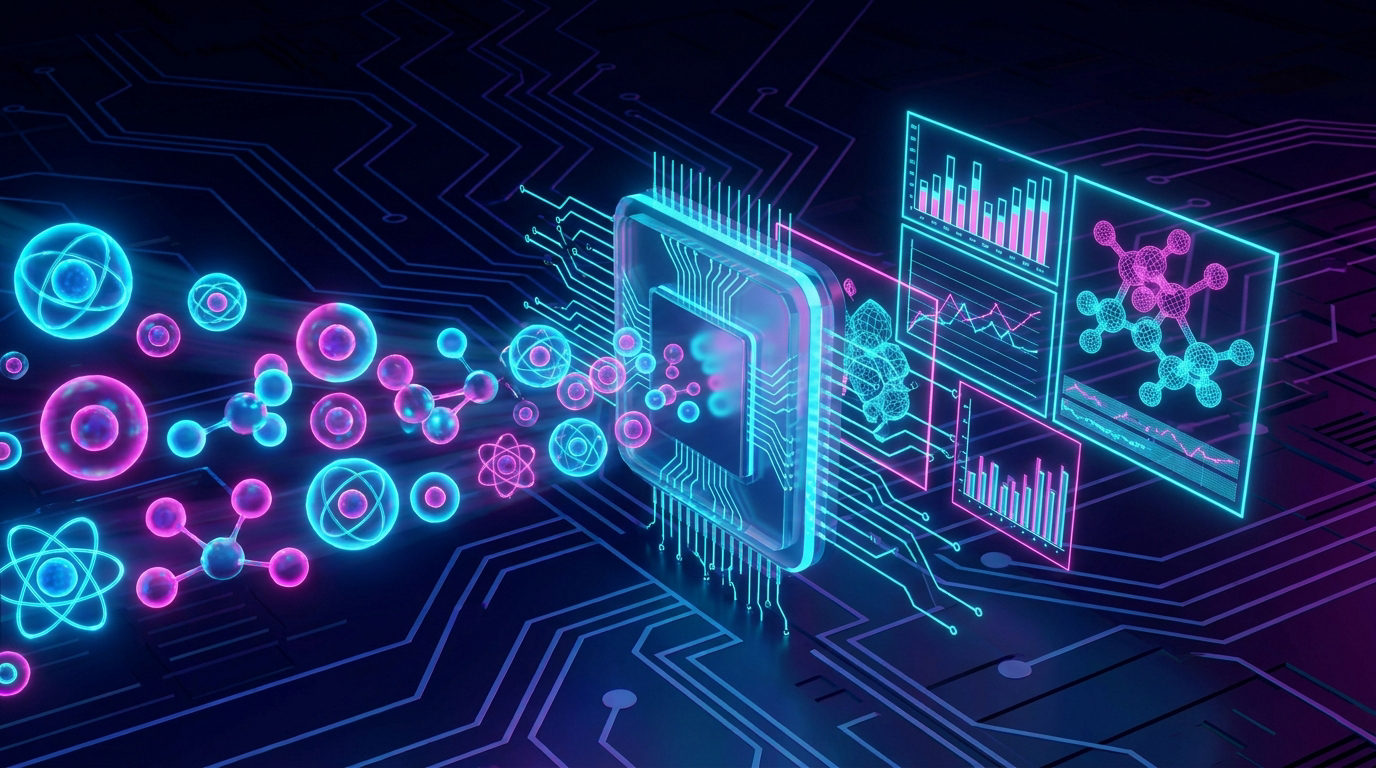
\includegraphics[width=0.5\linewidth]{assets/figures/ending_concept.png}}{}
	\end{center}
\end{frame}

\end{document}
